\section{Some discussion}

This chapter will contain most of the numerical error analysis and some of the discussion of this analysis as well as a recap of the methods used for error analysis in general, and how they are adapted to this particular problem.\\


In the numerical setup chosen for this project we will potentially introduce several new error sources in addition to the normal errors introduced by numerical solution of any equation (see section \ref{some_words_on_PDEs}). 
When a part of the solution acquired is replaced by the solution from a stochastic model, we will change the initial condition to the next iteration in time. 
This might have a number of effects on our final solution. 
Figure \ref{illustrate_approximate_derivatives} we can see the typical effects of solving an equation numerically. When we impose a stochastic solution on top of this again, we will get fluctuations around the approximations to the solution at the new time-step which most likely worsens our approximation.
The aim of this chapter is to verify our implementation and investigate the effects of adding the stochastic solution to the normal PDE solution.
% This can be done by choosing a solution to the PDE, doing a simulation which should yield the same solution and then comparing the two answers. 
% As argued in section \ref{} we will struggle with making the error from the random walk solver be much smaller than $\mathcal{O}(\Delta t)$. 
% We will therefore start by using a simple discretization of the PDE which also has a truncation error of $\mathcal{O}(\Delta t)$. 
% Figure \ref{errorplot_1d} shows the error norm (\ref{}) of only the PDE solver done in 1 dimension plotted for each timestep of the simulation. 
% The manufactured, exact solution is $u(x,t) = \exp\left(-\pi^2t\right)\cos(\pi x)$ and its initial condition is shown in figure \ref{}.

% \begin{figure}[H]
%  \centering
% %  \includegraphics[scale=0.7]{/home/fredriep/Dropbox/uio/thesis/doc/results/experiment_31102013_1017/results/initial_condition.eps}
%  \includegraphics[scale=0.7]{../doc/results/experiment_31102013_1017/results/initial_condition.eps}
%  \caption[Initial condition in 1d]{Initial condition of manufactured solution in 1d and the simulation.}
%  \label{initial_condition_1d}
% \end{figure}
% \begin{figure}[H]
%  \centering
% %  \includegraphics[scale=0.7]{/home/fredriep/Dropbox/uio/thesis/doc/results/experiment_31102013_1017/results/initial_condition.eps}
%  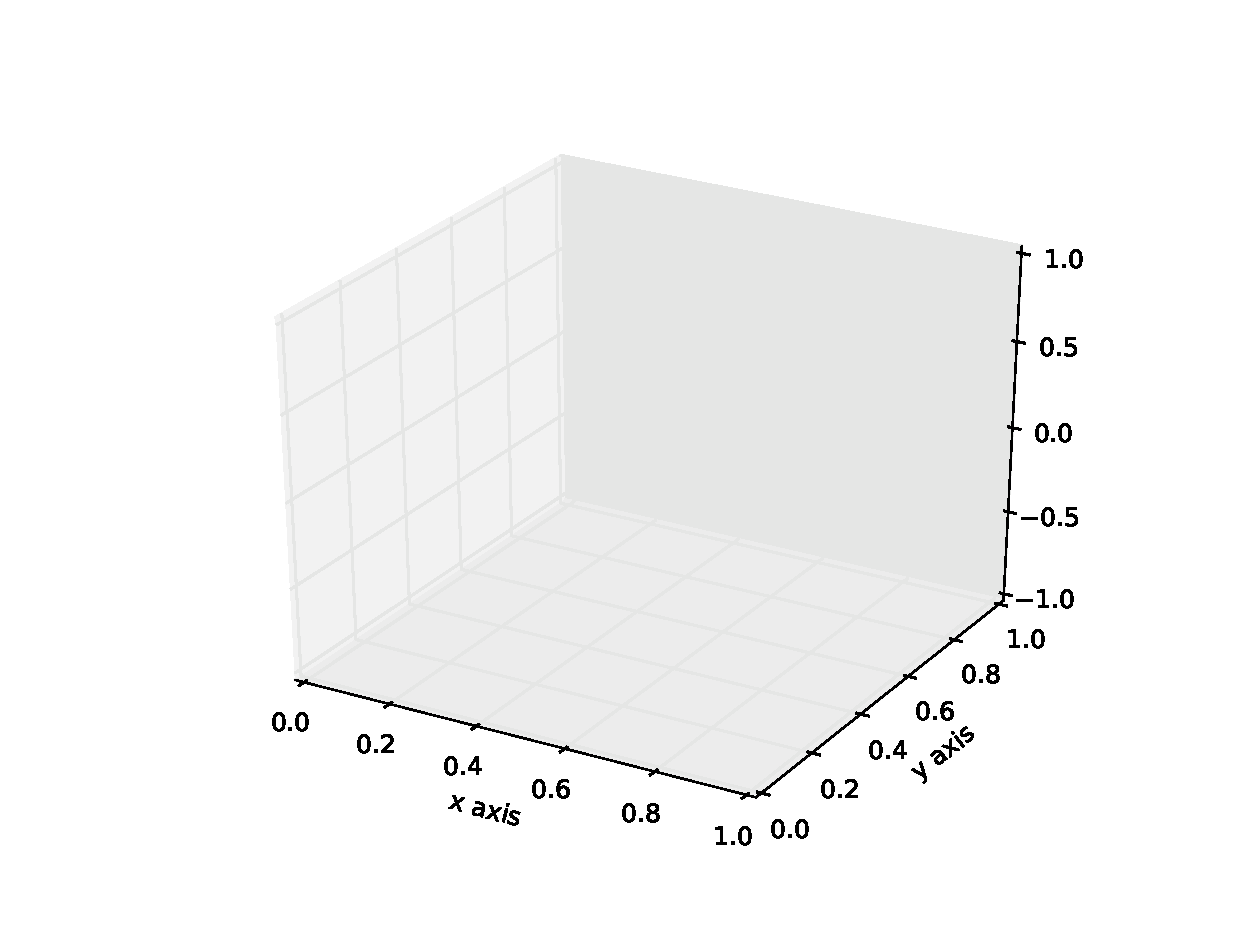
\includegraphics[scale=0.7]{Figures/InitialCondition2d.eps}
%  \caption[Initial condition in 2d]{Initial condition of manufactured solution in 2d and the simulation.}
%  \label{initial_condition_2d}
% \end{figure}

\subsection{The error estimate}\label{error_estimate}

Before we do anything we should specify what we use to measure the error which will be denoted as $\epsilon$. 
Throughout this thesis the term error is used quite lazily, but unless something else is specified we refer to the expression 
\begin{equation}
 \epsilon(t_i) = ||u_e(t_i)-u(t_i)||_2
\end{equation}
where $u_e$ is the exact (manufactured) solution to the equation, and $u$ is the result from the numerical simulation. 
We use this error-estimate because it is time-dependent, thus letting us explicitly see how the error evolves over time. 
The error is calculated over the entire mesh, letting us see clearly if the error from the random-walk areas are dominating, or (otherwise) how the PDE-scheme is holding up.
Another error estimate we will use later is the maximum value of the error. This will be used for the convergence tests to make sure that we overlook any effects of simulating for a long time. 
\begin{equation}
 \epsilon = max(\epsilon(t_i))
\end{equation}

\subsection{Verification techniques}
There are quite a few ways to verify an implementation. In this thesis we will focus on three which I think are adequate for no particular reason.
\begin{itemize}
 \item Method of manufactured solutions\\
 A normal way of checking that our scheme of choice is implemented correctly is by making an exact solution to the equation and checking that the error is of the expected order. 
Since the software contains both an explicit FE scheme and an implicit BE scheme we will verify the two of them alongside one another. 
We will start with the simplest diffusion equation (eq. \ref{simple_diffusion_equation}) and add complexity until we have the desired expression. 
Both schemes are expected to have an error-term of the order of $\Delta t$, which in the FE case is limited by a stability criterion. 
The next thing we do is decide that the solution to the diffusion equation should be equation \ref{manifactured_solution_1D} which satisfies our equation if we set the diffusion constant to 1. 
\item Exact numerical solutions\\
At least for the explicit schemes we can find an exact solution to the scheme itself seeing as the scheme is a difference equation. The calculations are shown step-by-step in chapter \ref{exact_numerical_solution}.
\item Convergence tests\\
This must be combined with the manufactured solution, but takes a slightly different approach to quantifying the error estimate. We start bu calculating some form of error estimate, and chose a value to represent the error of the entire simulation. This could be the maximum error for the entire simulation, or an integrated measure. 
We do multiple simulations while improving the parameter we want to investigate, say how the size of the time-step influences the error. 
Finally, using equation \ref{} we get a number indicating the improvement in the error estimate by improving the parameter in question. 
This number indicates the order of convergence which is one for FE and BE since the error goes as $\mathcal{O}(\Delta t)$, and two for our approximation to the second derivative in space since the error goes as $\mathcal O(\Delta x^2)$.
A convergence rate of 1 means that halving the parameter will (roughly) halve the error, while the same reduction for a second order convergence will reduce the error by 4.
\end{itemize}


\section{Verification of PDE solvers}
To verify the implementation of the PDE-solvers we will now run through the steps outlined in the previous chapter. 
We will also add complexity along the way, but this will be described when we get there. First of all we will test the simplest possible implementation which is equation \ref{}. 
Since both the FE and BE discretization have been implemented we will test both of them, but mostly we will use the BE discretization because it has no stability criterion. 
For most of the tests we will force the solution to be equation \ref{manifactured_solution_1D} in 1d which satisfies our equation if we set the diffusion constant to 1.

Despite testing the simple cases first we will do all the tests on the same implementation (the full one) because it should be able to recreate the simple cases as well. 
Setting $D(x,y) = 0.5$ as an array with all entries equal and inserting this into the schemes will return the average of $D(x,y)$ at different mesh-points, and effectively this is the same as having only a constant. 
We will also do all verification without random walkers.

\subsection{Manufactured Solutions}

As mentioned we force the solution to be equation \ref{manifactured_solution_1D} because it fulfills the boundary conditions we have chosen.
\begin{equation}\label{manifactured_solution_1D}
 u(x,t) = e^{-t\pi^2}\cos(\pi x) +1
\end{equation}
Equations \ref{manufactured_prof_pt1} and \ref{manufactured_prof_pt2} prove that the manufactured solution we have chosen will indeed fulfill the diffusion equation (eq. \ref{simple_diffusion_equation}).
\begin{align}
 \frac{\d }{\d t}e^{-t\pi^2}\cos(\pi x) +1 &= D\frac{\d^2}{\d x^2}e^{-t\pi^2}\cos(\pi x) +1\label{manufactured_prof_pt1}\\
 -\pi^2e^{-t\pi^2}\cos(\pi x) &= -\pi^2e^{-t\pi^2}\cos(\pi x) +1 \implies 1 = 1\label{manufactured_prof_pt2}
\end{align}

The error in space is determined by two factors, the actual error caused by the approximation to the second derivative, which is of the order of $\Delta x^2$ and, in the FE case, the error term coming from the time derivative due to the stability criterion (eq. \ref{stability}), which is also of the order $\Delta x^2$. 
In 1D we get the plots in figure \ref{errorplot_FE1D_noWalk} of error described in chapter \ref{error_estimate}, with the corresponding plots of the convergence rates in figure \ref{} that verify the order of the error term.
For longer simulations, we expect the analytic solution to reach a steady state which we find in the limit of large $t$. 

\begin{equation}
 u(x,t\to\infty) \to e^{-\infty}\cos(\pi x) +1 \to 1
\end{equation}
The numerical scheme should be able to represent this to machine precision ($10^{-16}$), meaning that the numerical solution should start converging to zero after some number of times steps, but this might depend on how the derivatives as estimated so we say that it should in the very least stabilize. 
Figures \ref{} and \ref{} seem to show the expected behaviour from the error estimate, which implies that the implementation is correct so far.

\begin{figure}[H]
\centering
\begin{subfigure}[b]{0.48\textwidth}
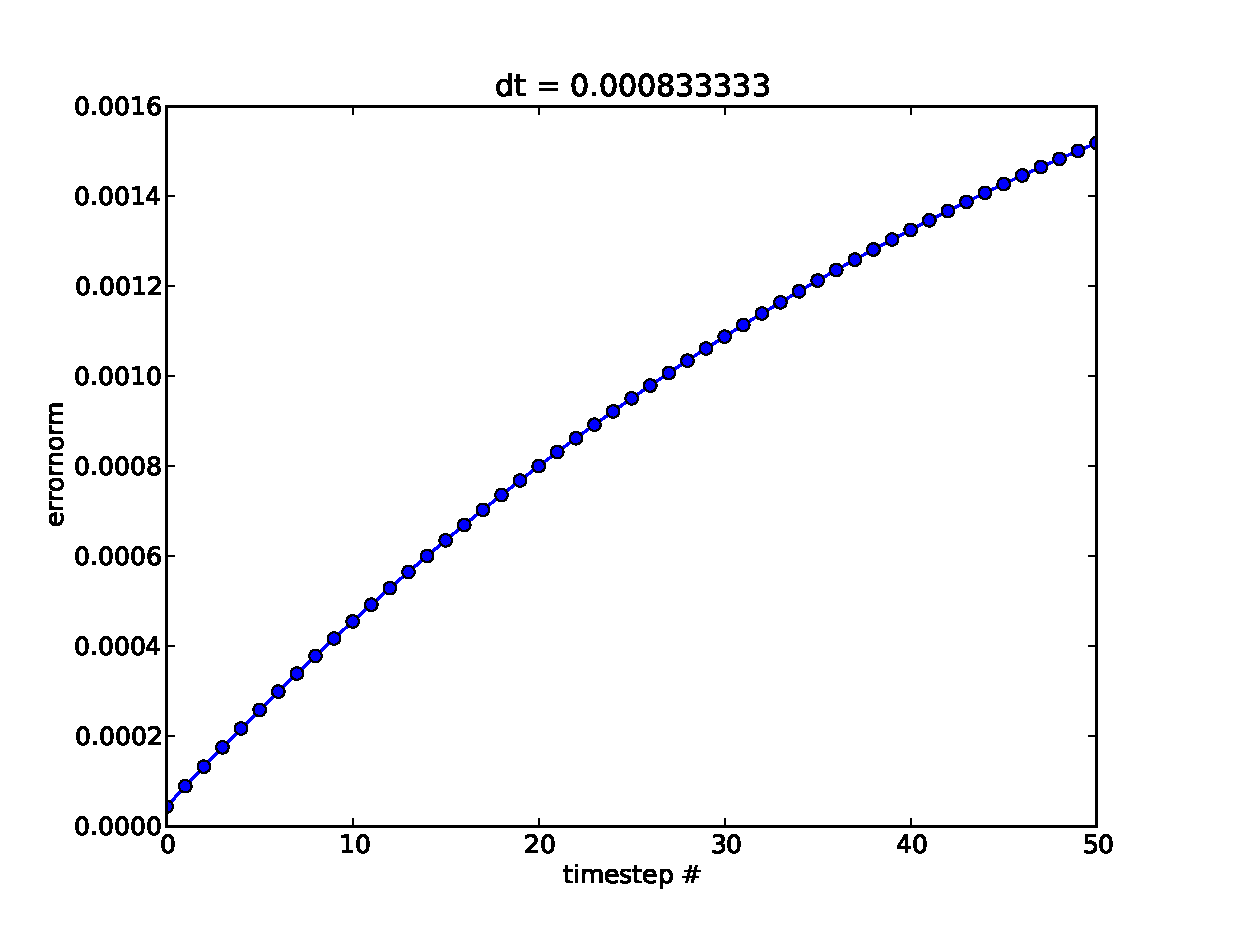
\includegraphics[width=\textwidth]{../doc/results/experiment_31102013_1017/results/deterministic_errorplot.eps}
\caption{}
\label{errorplot_FE1D_noWalk}
\end{subfigure}
\begin{subfigure}[b]{0.48\textwidth}
 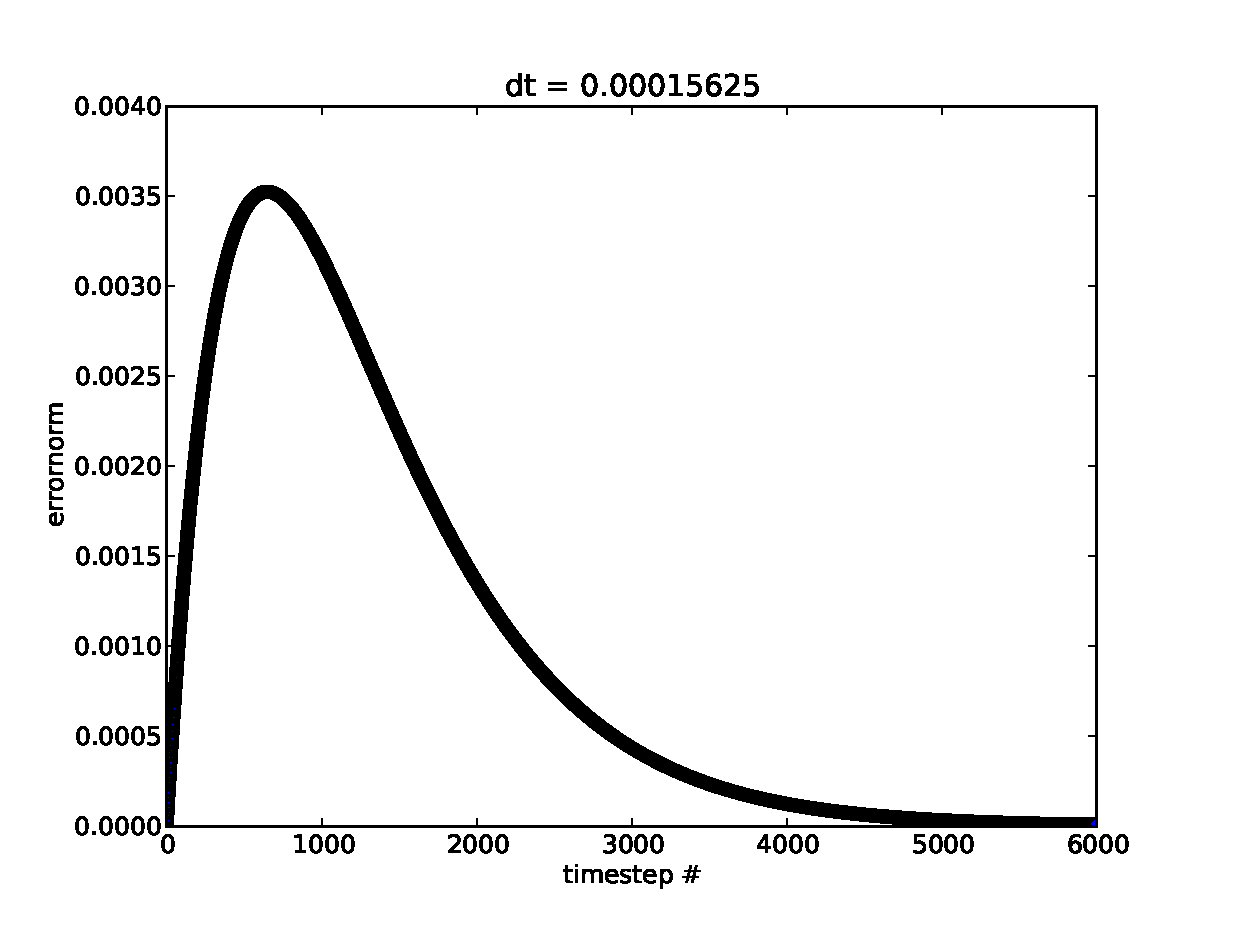
\includegraphics[width=\textwidth]{../doc/results/experiment_18112013_0830/results/deterministic_errorplot.eps}
 \caption{}
 \label{errorplot_FE1D_noWalk_long}
\end{subfigure}
\caption[Numerical error for 1D Forward Euler discretization]{Numerical error for 1D Forward Euler discretization of the PDE. Nothing else is done to the simulation.}
\label{errorplot_FE1D_noWalk_super}
\end{figure}

As we discussed in section \ref{random_walks_and_anisotropy} we should also be able to model diffusion where the diffusion constant is not a constant. 
The scheme we derived in section \ref{discretizing} already takes this into account, and so all we need to do is to add the drift term which was discussed in section \ref{effect_of_drift_on_walkers} to the scheme. 
Like before we should verify that the scheme solves the equation to the expected accuracy by using a manufactured solution \ref{manifactured_solution_1D} and tweaking the source term so this function solved the equation \ref{convection_diffusion_equation}. 
When $v=0$ and $D(x) = \pi x$ the source term becomes
\begin{align*}
 -\pi^2\exp\left(-\pi^2t\right)\cos\left(\pi x\right) &= -\pi\exp\left(-\pi^2t\right)\frac{\d}{\d x}\pi x\sin(\pi x) +f(x,t) \\
 -\pi^2\cos\left(\pi x\right) &= -\pi^2\left(\sin(\pi x) + \pi x\cos(\pi x)\right) +\tilde{f}(x) \\
 \tilde{f}(x) &= \pi^2\left(\sin(\pi x) +\cos(\pi x)(\pi x-1)\right)
\end{align*}
Once again $f(x,t) = \exp\left(-\pi^2t\right)\tilde{f}(x)$. Figure \ref{anisotropic_diffusion_verification} shows the error norm of the result of simulations of this equation with different values of $\Delta t$.

\begin{figure}[H]
\centering
\begin{subfigure}[b]{0.48\textwidth}
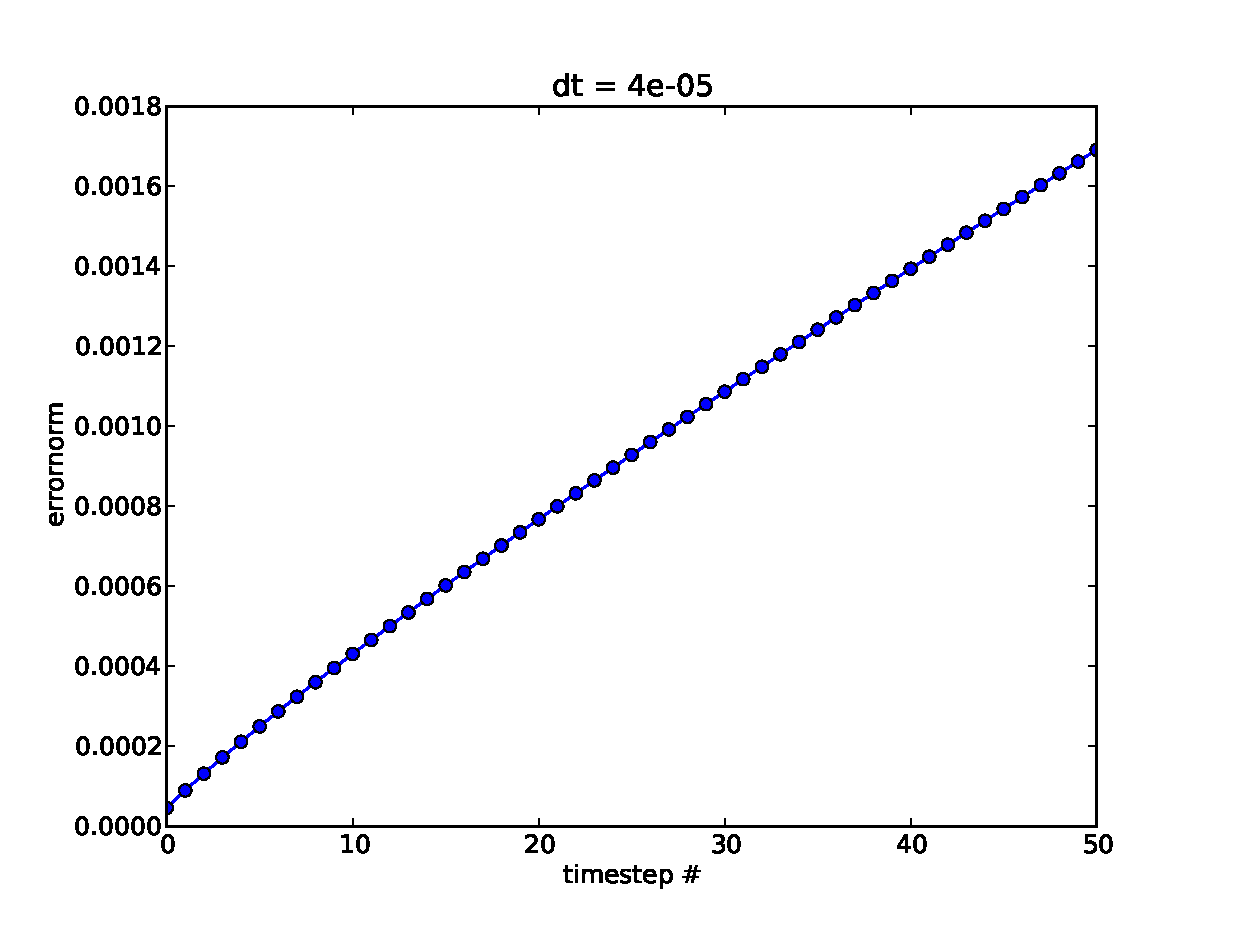
\includegraphics[width=\textwidth]{../doc/results/experiment_05112013_1303/results/deterministic_errorplot.eps}
\caption{}
\label{anisotropic_diffusion_verification:single_dt}
\end{subfigure}
\begin{subfigure}[b]{0.48\textwidth}
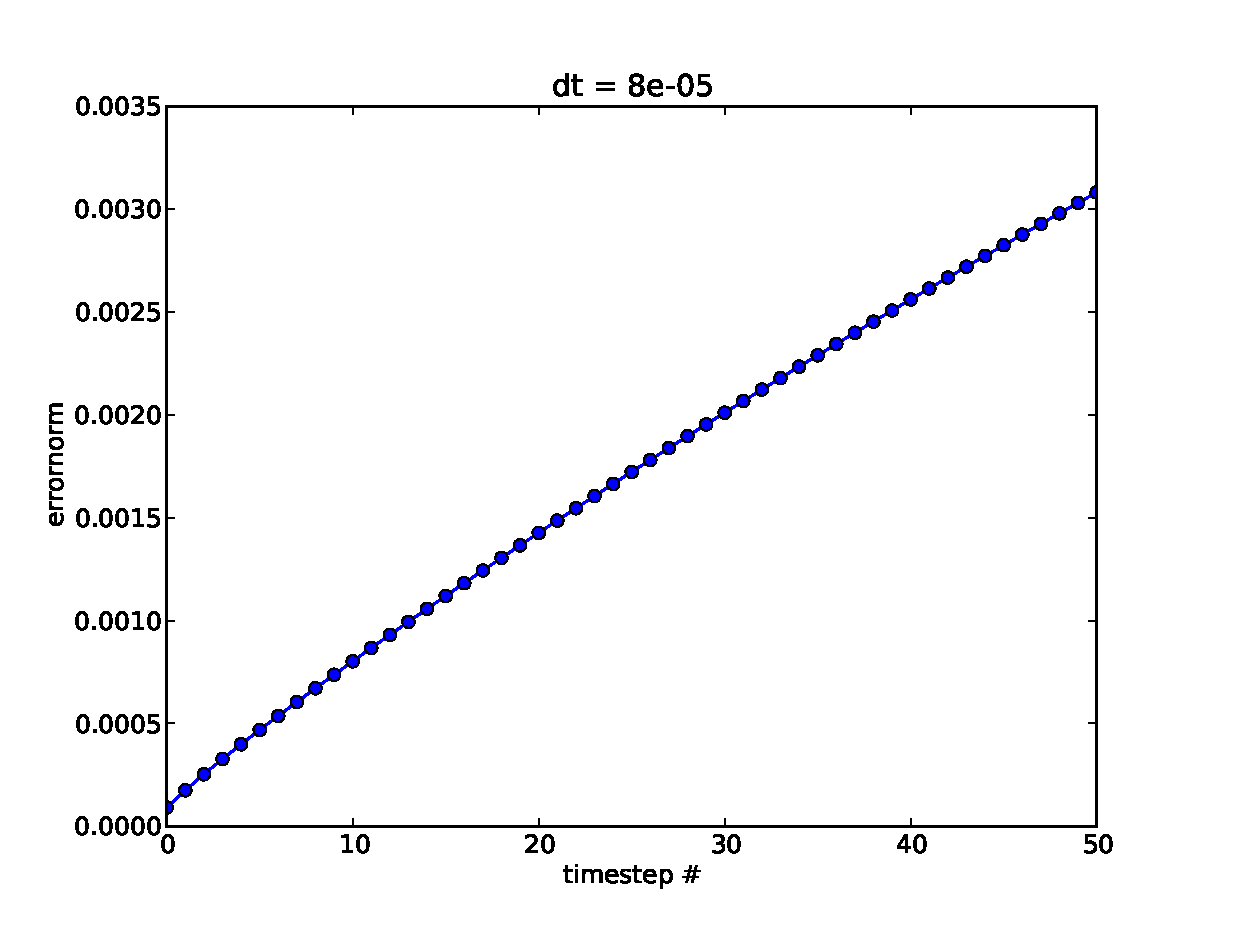
\includegraphics[width=\textwidth]{../doc/results/experiment_05112013_1304/results/deterministic_errorplot.eps}
\caption{}
\label{anisotropic_diffusion_verification:double_dt}
\end{subfigure}
\caption[Verification of anisotropic diffusion equation implementation]{Verification of anisotropic diffusion equation implementation}
\label{anisotropic_diffusion_verification}
\end{figure}
Again, the error is of the order of $\Delta t$ and is roughly halved by halving $\Delta t$.

\subsection{Convergence Tests}

The next step in testing the implementation will be to perform a convergence test in time. 
We omit the spatial convergence test because chances are very good that an incorrect implementation of the spatial derivative would be clearly visible both in the visualization of the simulation (the solution blows up), and in the error plot seeing as the spatial error would dominate.
We carry out the convergence test by doing several simulations with different values for $\Delta t$ and comparing the errors by equation \ref{convergence_rate_def}. 
A result of such an experiment for the FE scheme using the $\Delta t$ values listed below is found in figure \ref{convergence_test_FE}. 
The expected value of r is approximately 1. The result is not perfect, but still close to 1. 
For the BE scheme we get the convergence rate shown in figure \ref{convergence_test_BE}. Again, the expected order of convergence is 1 and this time the result is almost perfect.
\begin{lstlisting}
 dt = [1e-4,1e-5,1e-6,1e-7,1e-8]
\end{lstlisting}
\begin{figure}[H]
 \centering
 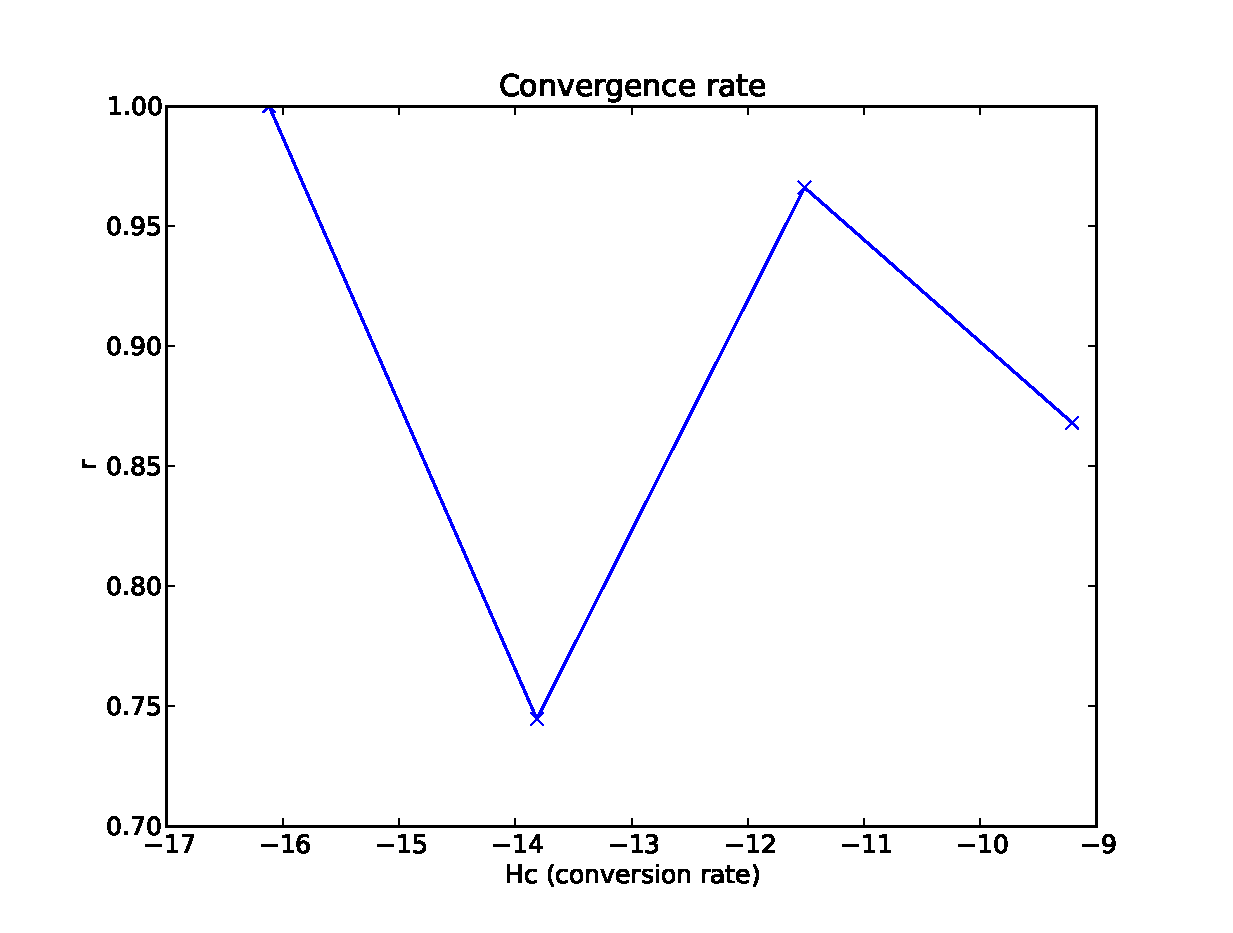
\includegraphics[scale=0.7]{../doc/results/experiment_27112013_1017/results/ConvergenceTest.eps}
 \caption{Convergence test for the FE scheme. The x axis is $\ln(\Delta t)$.}
 \label{convergence_test_FE}
\end{figure}
\begin{figure}[H]
 \centering
 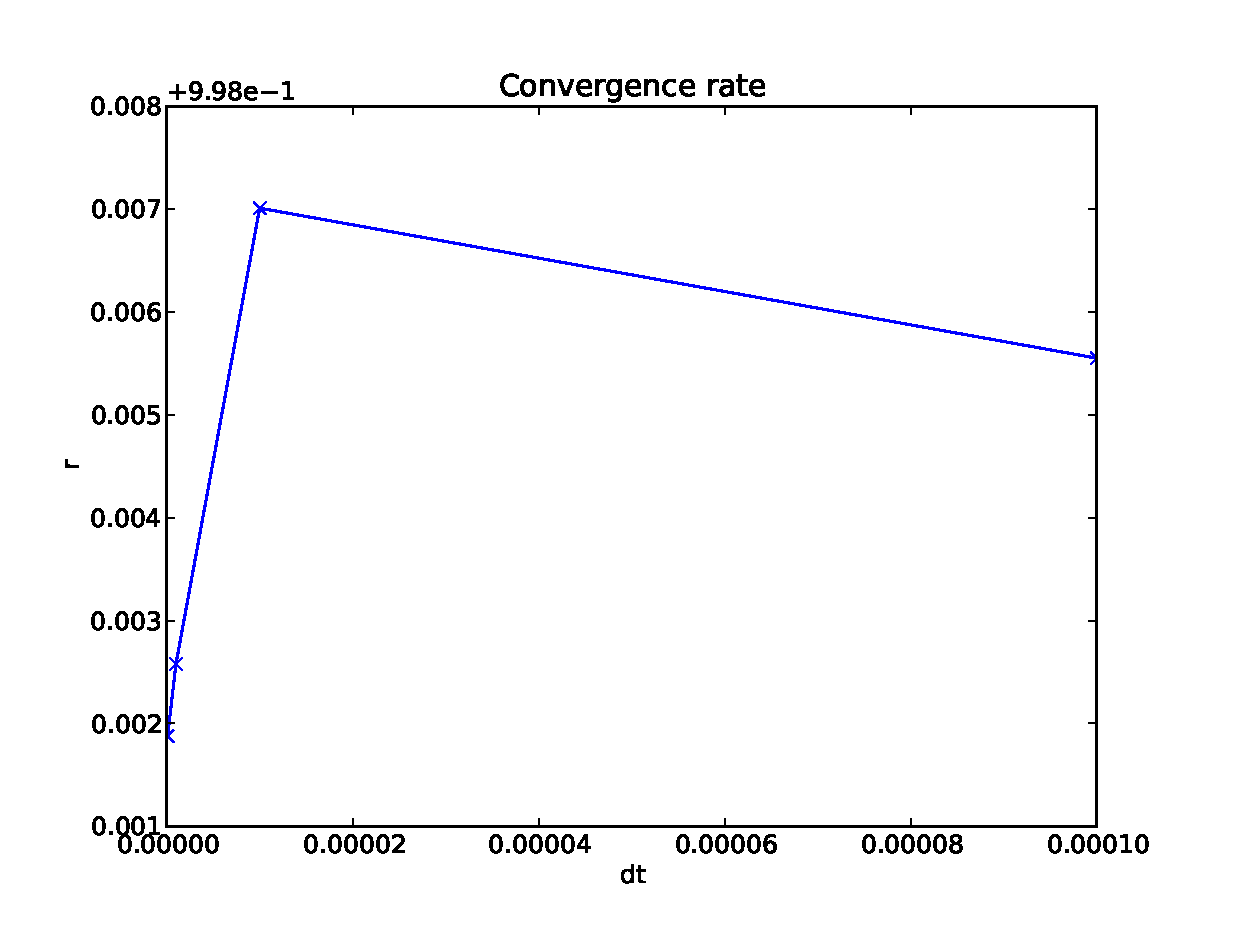
\includegraphics[scale=0.7]{../doc/results/experiment_13012014_0925_Simple1DConvergenceTestBE/results/ConvergenceTest.eps}
 \caption{Convergence test for the BE scheme. The x axis is $\Delta t$, the y-axis (though a little hard to see) is zoomed in around r=1.}
 \label{convergence_test_BE}
\end{figure}

We can also do a convergence test, equal to the one we did in 1d, to check that the scheme converges to 1 (by equation \ref{convergence_rate_def}) for smaller $\Delta t$. 
The results of this test are shown in figure \ref{convergence_test_FE_2d} and it does converge nicely to one.

\begin{figure}[H]
\centering
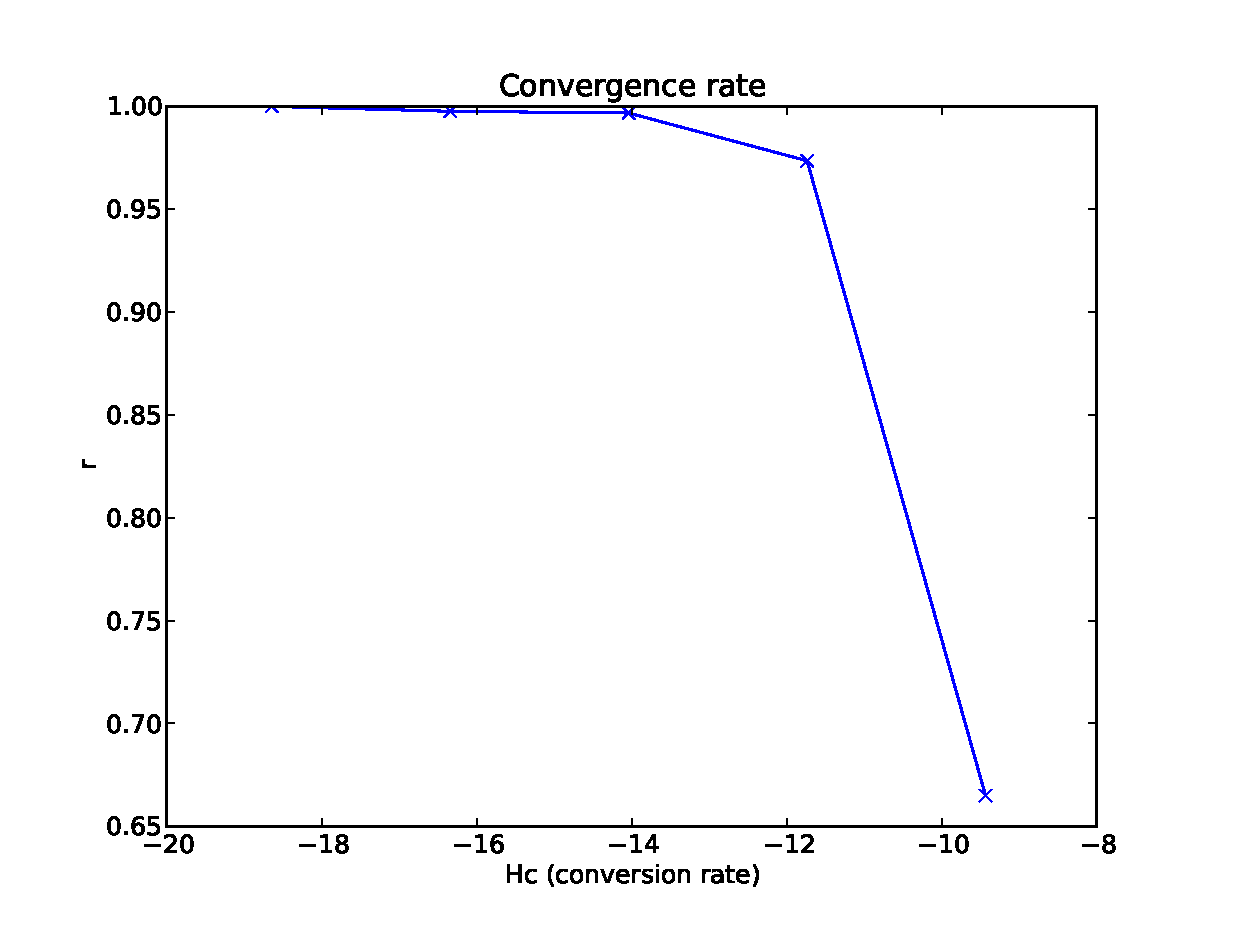
\includegraphics[scale=0.7]{../doc/results/experiment_29112013_1709/results/ConvergenceTest.eps}
\caption[Convergence test FE 2d]{Convergence test for the FE scheme in 2d using $\Delta t$ ranging from the stability criterion $\frac{\Delta x\Delta y}{5}$ to the same ratio divided by 100000 in increments of $10^{-1}$.}
\label{convergence_test_FE_2d}
\end{figure}

\subsection{Exact numerical solution}\label{exact_numerical_solution}

The FE scheme also has an exact solution seeing as it is in fact a difference equation. 
We can find this (for this exact initial condition, eq. \ref{manifactured_solution_1D}) if we formulate the scheme as 

\begin{equation}
 u^{n+1} = D\Delta t u_{xx}^n + u^n
\end{equation}

and insert for the first few iterations. 

\begin{align*}
 u^1 &= D\Delta t u_{xx}^0 + u^0 \\
 u^2 &= D\Delta t u_{xx}^1 + u^1 = D\Delta t\left[D\Delta t u_{4x}^0 + u_{2x}^0\right] + u^0\\
 &= \left(D\Delta t\right)^2 u_{4x}^0 + 2D\Delta t u_{2x}^0+ u^0 \\
 u^3 &= D\Delta t u_{xx}^2 + u^2 = D\Delta t\left[\left(D\Delta t\right)^2 u_{6x}^0 + 2D\Delta t u_{4x}^0+ u_{2x}^0\right] + \left(D\Delta t\right)^2 u_{4x}^0 + 2D\Delta t u_{2x}^0+ u^0\\
 &= \left(D\Delta t\right)^3 u_{6x}^0 + 3\left(D\Delta t\right)^2 u_{4x}^0+ 3D\Delta tu_{2x}^0 + u^0 \\
 u^4 &= D\Delta t u_{xx}^3 + u^3 = \dots \\
 &= \left(D\Delta t\right)^4 u_{8x}^0 + 4\left(D\Delta t\right)^3 u_{6x}^0+ 6\left(D\Delta t\right)^2 u_{4x}^0 + 4D\Delta t u_{2x}^0 + u^0 
\end{align*}
Which we can generalize to 
\begin{equation}
 u^{n+1} = \sum\limits_{i=0}^n {n\choose i}\left(D\Delta t\right)^iu^0_{2ix}
\end{equation}
where we have
\begin{equation*}
 u^0_{2ix} = \left(-1\right)^i\pi^{2i}\cos(\pi x)
\end{equation*}
from the initial condition. This finally gives us the exact numerical solution of the FE scheme in time. 
\begin{equation}
 u^{n+1} = \sum\limits_{i=0}^n {n\choose i}\pi^{2i}\left(-1\right)^i\left(D\Delta t\right)^i\cos(\pi x)
\end{equation}

Notice that we have not used the approximation to the spatial derivative, but rather the analytical derivative. 
We can find the approximation that the computer uses to the spatial derivative in the same way as for the time derivative. 
\begin{align*}
 u^0_{xx} &= \frac{1}{\Delta x^2}\left(\cos(\pi(x+\Delta x)) -2\cos(\pi x) +\cos(\pi(x-\Delta x))\right) \\
 &= \frac{2}{\Delta x^2}\left(\cos(\pi\Delta x)-1\right)\cos(\pi x)\\
 u^0_{4x} &= [u^0_xx]_{xx} = \frac{1}{\Delta x^2}\left[\frac{2}{\Delta x^2}\left(\cos(\pi\Delta x)-1\right)\left(\cos(\pi(x+\Delta x)) -2\cos(\pi x) +\cos(\pi(x-\Delta x))\right)\right]\\
 &= \frac{4}{\Delta x^2}\left(\cos(\pi\Delta x)-1\right)^2\cos(\pi x)\\
 &\dots
\end{align*}
We can immediately see that this pattern continues, and we get the general formula in equation \ref{numerical_solution} for the exact numerical solution.
\begin{equation}\label{numerical_solution}
  u^{n+1} = \sum\limits_{i=0}^n {n\choose i}\left(D\Delta t\right)^i\frac{2^i}{\Delta x^{2i}}\left(\cos(\pi\Delta x)-1\right)^i\cos(\pi x)
\end{equation}
We expect the FE scheme to represent this solution more or less to machine precision, at least to $15$ digits. 
There are, however two issues with the solution \ref{numerical_solution}:
\begin{itemize}
 \item $\Delta x^{2i}$ will quickly tend to zero, and the computer will interpret it as zero. This will cause division by zero, which again ruins the simulation. This can be fixed rather simply by testing if $\Delta x^{2i}>0$ and returning zero if the test returns false.
 \item ${n\choose i}$ goes to infinity for large n and i. We will eventually (for $n>\sim170$) meet overflow. Figure \ref{convergence_exact_numerical_1d_n145} shows that at least for relatively few time steps  we can drop the troublesome terms.
\end{itemize}

\begin{figure}[H]
 \centering
 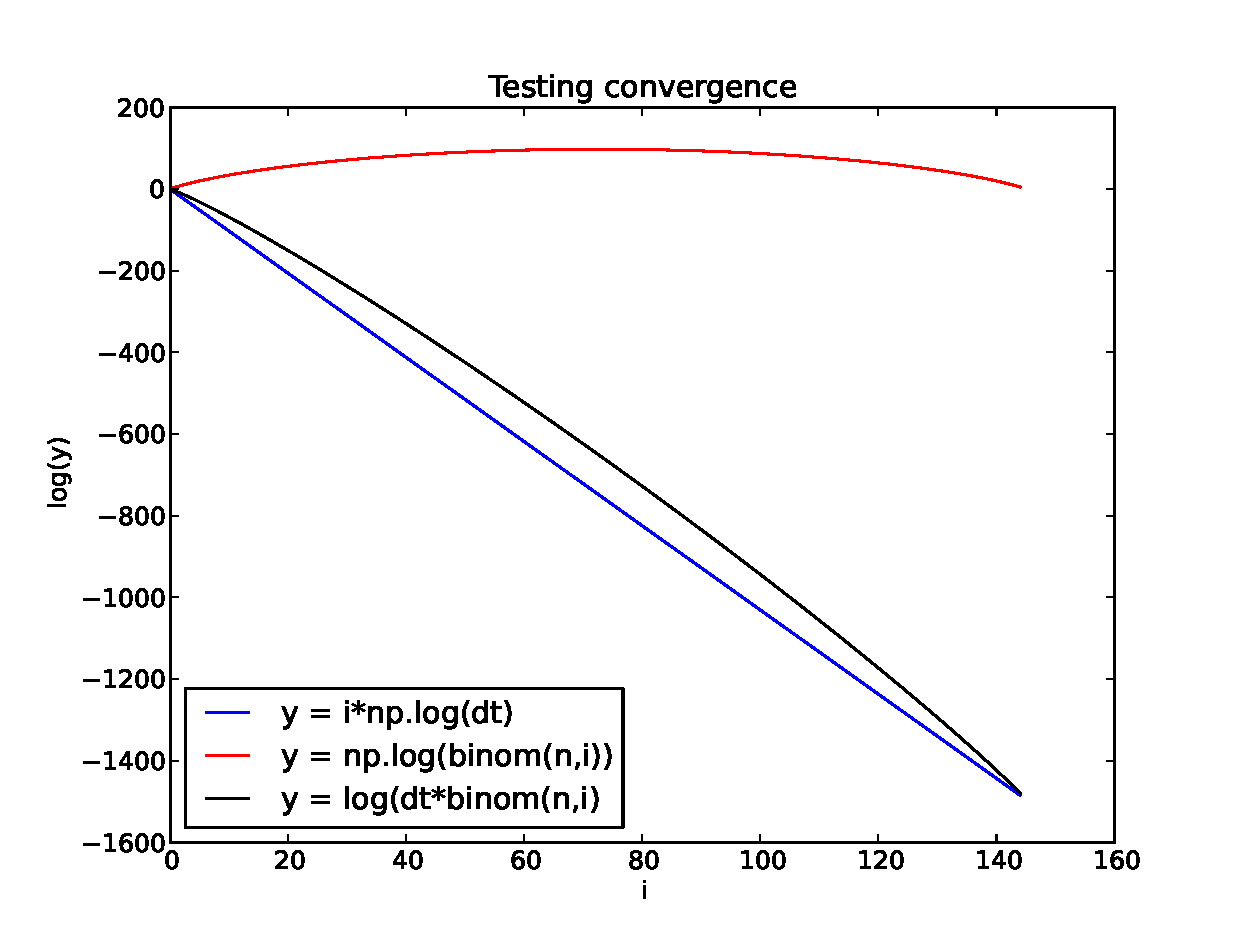
\includegraphics[scale=0.7]{Figures/convergence_exact_numerical_1d_n145}
 \caption{Testing the relation between $\left(D\Delta t\right)^i$ and the binomial coefficients.}
 \label{convergence_exact_numerical_1d_n145}
\end{figure}
The results from testing the FE scheme are found in figure \ref{errorplot_numerical_exact_FE_1D}. We see that the error in the worst case is about an order of magnitude worse than we expected. This is most likely due to the fact that we are cutting part of the solution, and over several time steps the error we do might accumulate.

\begin{figure}[H]
 \centering
 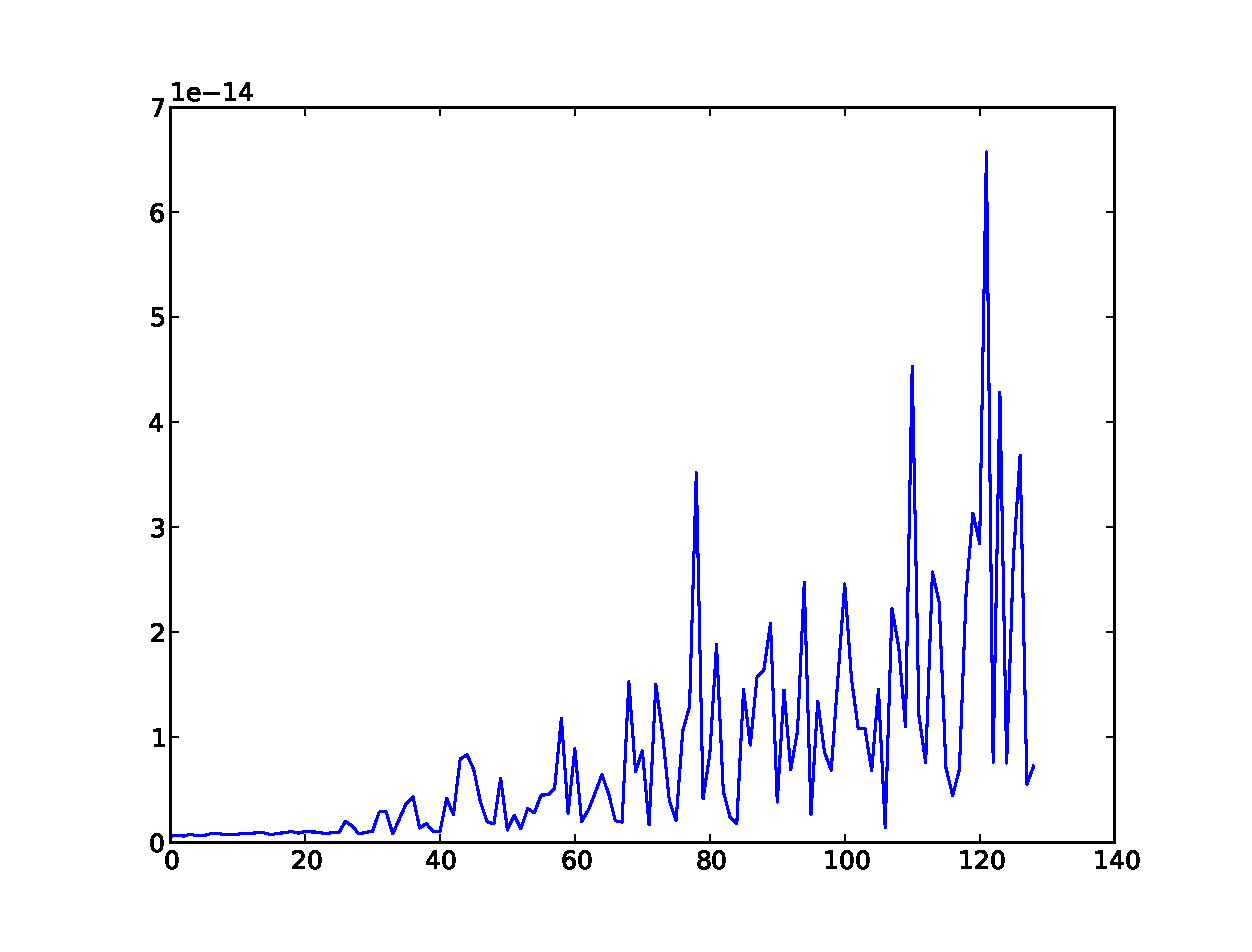
\includegraphics[scale=0.7]{Figures/exact_numerical_1d_n130.eps}
 \caption[Verification for exact numerical solution]{Error plot for 1d FE scheme compared to the exact numerical solution \ref{numerical_solution} with the modifications suggested earlier.}
 \label{errorplot_numerical_exact_FE_1D}
\end{figure}
Doing the same tests is 2D gives slightly different results; adding a 2D walk-domain has an influence on the error, but a rather small one. 
This can, however be tweaked by increasing the conversion parameters.

\begin{equation}\label{initial_condition_2d_numex}
 u(x,y,t=0) = \cos(\pi x)\cos(\pi y)
\end{equation}

The exact numerical solution of the FE scheme can be found in equation \ref{exact_numerical_solution_2d}, and again we expect the scheme to be able to reproduce this to more or less machine precision. 
The result of a test simulation of this, using the initial condition in equation \ref{initial_condition_2d_numex}, is shown in figure \ref{exact_numerical_2d_n130}. 
Again, as in we did in 1d, we see that although the error is very small, and start out with machine precision, it does increase and even more than in the 1d case. 
This is \emph{probably} because of the terms we have do drop in the exact numerical solution due to overflow and so on, which accumulate in the numerical solution from the scheme. 
We should, in other words, be pleased that the error starts out with machine precision, and stays small for the amount of time steps we can simulate and still have something to compare it with.

\begin{equation}\label{exact_numerical_solution_2d}
 u^{n+1} = \sum\limits^n_{i=0}{n\choose i}\left(D\Delta t\right)^i\left[2^{i-1}\cos(\pi x)\cos(\pi y)\left(\frac{(\cos(\pi\Delta x))^i}{\Delta x^{2i}} +\frac{(\cos(\pi\Delta y))^i}{\Delta y^{2i}}\right)\right]
\end{equation}

\begin{figure}[H]
 \centering
 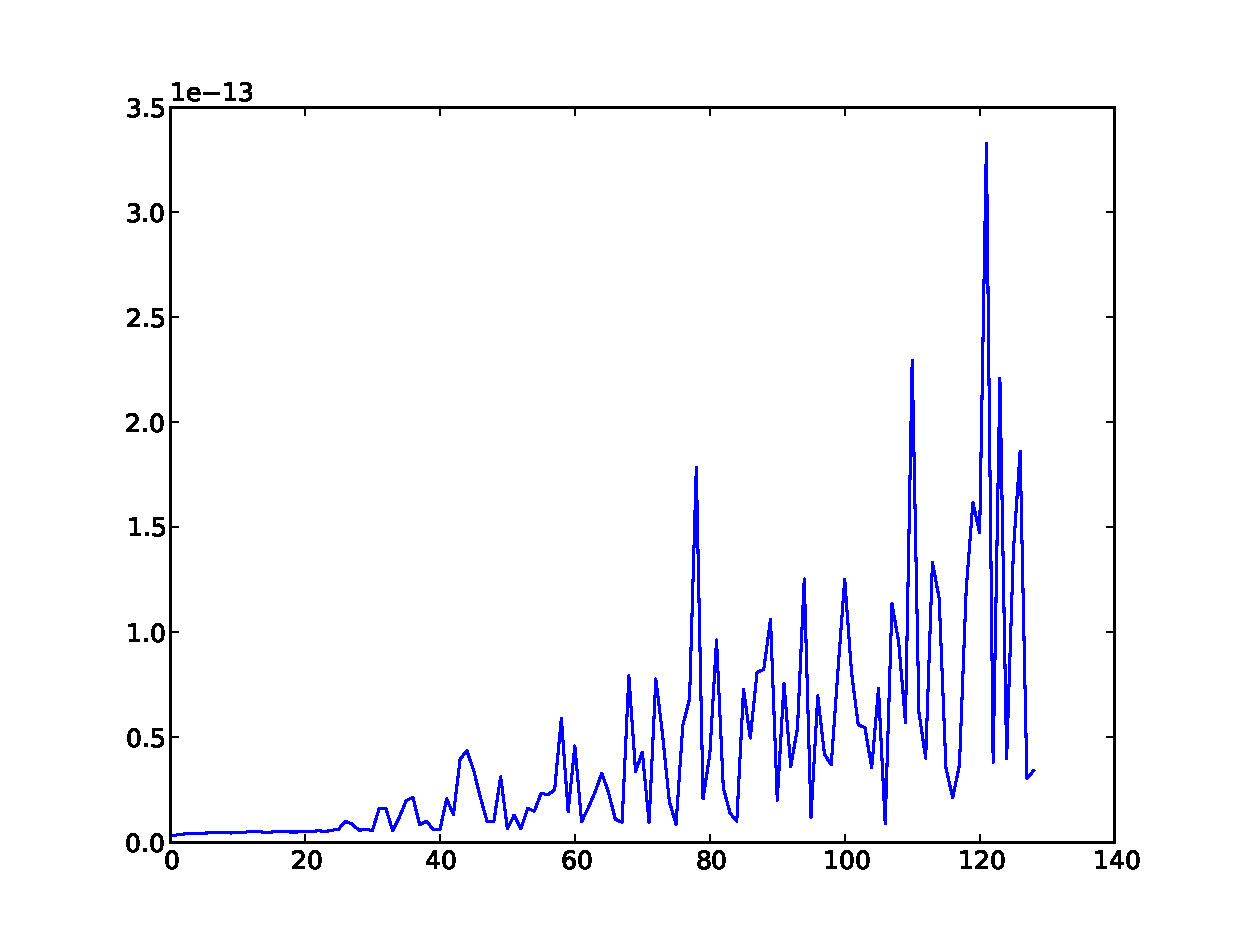
\includegraphics[scale=0.7]{Figures/exact_numerical_2d_n130.eps}
 \caption{Numerical solution from the FE scheme versus the exact numerical solution of the FE scheme in 2d. we have used a $\Delta t$ which is almost on the stability criterion, $\Delta t = \frac{\Delta x \Delta y}{5} = 8e-05$.}
 \label{exact_numerical_2d_n130}
\end{figure}

\section{Testing the Random walk implementation}\label{testing_random_walks}



To verify our implementation, and perhaps gain some new knowledge we will do some testing on the random walks implementation as well. 
This means that we have to find a solution of the diffusion equation \ref{simple_diffusion_equation} for an initial condition we can recreate with random walkers to the best possible precision. 
The absolute simplest initial condition to recreate is the Heaviside step function, defined in equation \ref{Heaviside_def}. 
\begin{equation}\label{Heaviside_def}
 H(x-a) = \begin{cases}
           1\;\;x\geq a\\
           0\;\;x<a
          \end{cases}
\end{equation}
In order to verify our implementation we must solve the diffusion equation \ref{simple_diffusion_equation} for this new initial condition. 
This is most easily done through separation of variables. We have
\begin{align*}
 \frac{\d u}{\d t} = D\frac{\d^2 u}{\d x^2};\;\; \frac{\d u(0,t)}{\d x} = \frac{\d u(1,t)}{\d x} = 0 \\
 u(x,0) = H\left(x-\frac{1}{2}\right);\;\; D = 1
\end{align*}
and
\begin{align*}
 u(x,t) = F(x)T(t) \implies \frac{T'(t)}{T(t)} = \frac{F''(x)}{F(x)}
\end{align*}
where the primes denotes the respective derivatives. We separate the equation using a separation constant $\lambda$
\begin{align*}
 T'(t)-\lambda T(t) = 0 \implies T(t) = C\exp(\lambda t)\\
 F''(x) -\lambda F(x) = 0 \implies F(x) = C_1\exp(\sqrt{\lambda}x) + C_2\exp(-\sqrt{\lambda}x)
\end{align*}
Where $C$, $C_1$ and $C_2$ are arbitrary constants. 
Choosing $\lambda = -\mu^2$ lets us rewrite the spatial solution in terms of sines and cosines
\begin{equation*}
 F(x) = a\cos(\mu x) + b\sin(\mu x)
\end{equation*}
The boundary conditions gives us 
\begin{align*}
 F'(0)T(t) = F'(1)T(t) = 0
\end{align*}
Since the time dependent solution cannot be exactly zero, the first derivative of the spatial solution must be zero
\begin{align*}
 F'(x) &= -a\mu\sin(\mu x) + b\mu\cos(\mu x) \\
 F'(0) &= -a \mu\sin(0) + b\mu\cos(\mu x) = b\mu\cos(\mu x) \implies b=0 \\
 F(1) &= a\cos(\mu) \implies \mu = n\pi
\end{align*}
Telling us that a Fourier series in cosines is the solution to the equation, and it will look like this.
\begin{equation}
 u(x,t) = a_0 + \sum\limits_{n=1}^\infty a_n\exp\left(-(n\pi)^2t\right)\cos(n\pi x)
\end{equation}

The coefficients are found by approximating the initial condition
\begin{align*}
 a_0 &= \int\limits_0^1H(x-0.5)dx = \frac{1}{2} \\
 a_n &= 2\int\limits_0^1H(x-0.5)\cos(n\pi x)dx = 2\int\limits_{0.5}^1\cos(n\pi x)dx \\
 &= \frac{2}{n\pi}\left[sin(n\pi x)\right]_{0.5}^1 = \frac{2}{n\pi}\sin(n\pi) - \sin(\frac{n\pi}{2}) \\
 a_n &= \frac{2\sin(\frac{n\pi}{2})}{n\pi}
\end{align*}
which gives us the final solution
\begin{equation}
 u(x,t) = \frac{1}{2} + \sum\limits_{n=1}^\infty \frac{2\sin(\frac{n\pi}{2})}{n\pi}\exp\left(-(n\pi)^2t\right)\cos(n\pi x)
\end{equation}

We can now perform a convergence test to find the convergence rate for the random walkers, this is the order the error of the scheme goes as and it is defined in equation \ref{convergence_rate_def}. 
We will modify it slightly by testing for the number of walkers rather than the time step. 
We must also use another error estimate $E_i$ which gives us one number for each simulation. 
The candidates are either the maximum of the error we are already using, or an integrated error.

\begin{equation}\label{convergence_rate_def}
 r = \frac{\ln(E_{i+1}/E_i)}{\ln(\Delta t_{i+1}/\Delta t_i)}
\end{equation}

Using the maximum of the error measure already in use, we have tested the convergence rate measure for the following measures of Hc:
\begin{lstlisting}
 Hc = [200,1400,5600,10400,32000]
\end{lstlisting}
Meaning that the largest value of Hc we will get an estimate for is $Hc = 10000$. 
The convergence test suggests that the convergence rate for random walks follows the proportionality in equation \ref{convergence_rate_RW}. 
This relation tells us just what we have been expecting the whole time; while increasing the number of walkers will reduce the error, the convergence is slow. 
Should we wish to do so, we can force the error to $\mathcal{O}(\Delta t^2)$, but this will be extremely inefficient. In fact we can find the relation as $Hc\sim\Delta t^{-2}$ for $err\sim\mathcal{O}(\Delta t)$, and $Hc\sim\Delta t^{-4}$ for $err\sim\mathcal{O}(\Delta t^2)$. Clearly we will have enough trouble for the simpler cases.

\begin{equation}\label{convergence_rate_RW}
err \propto Hc^{\frac{-1}{2}}
\end{equation}


\begin{figure}[H]
 \centering
 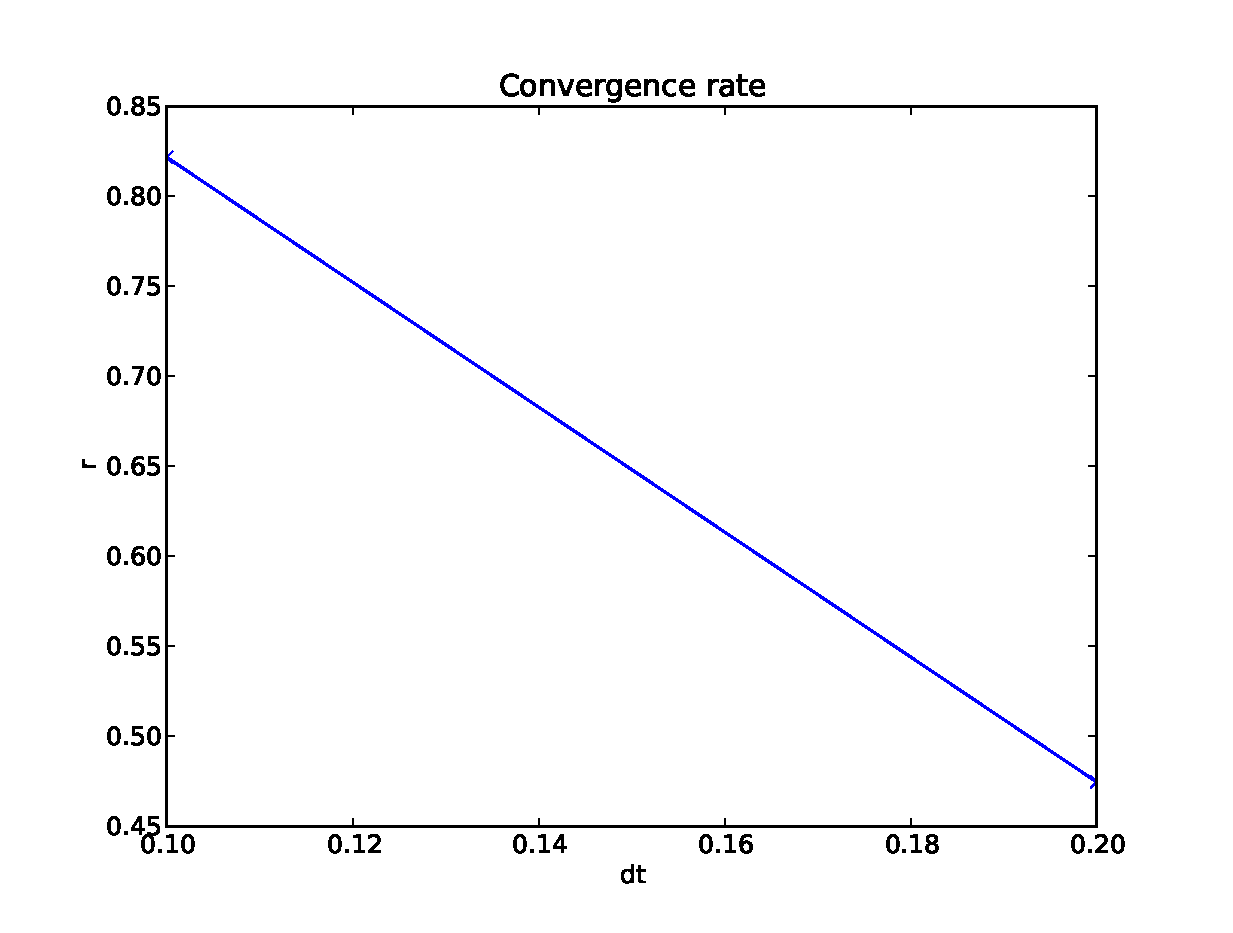
\includegraphics[scale=0.7]{../doc/results/experiment_18022014_1413_RW_convergencetest_1d/ConvergenceTest.eps}
 \caption[Convergence test RW]{A convergence test for the isotropic random walk implementation using different conversion factors, Hc. The x axis (conversion rate) is log transformed and ranges from 100 to 50000 in real numbers.}
 \label{ConvergenceTestRW}
\end{figure}
\begin{figure}[H]
 \centering
 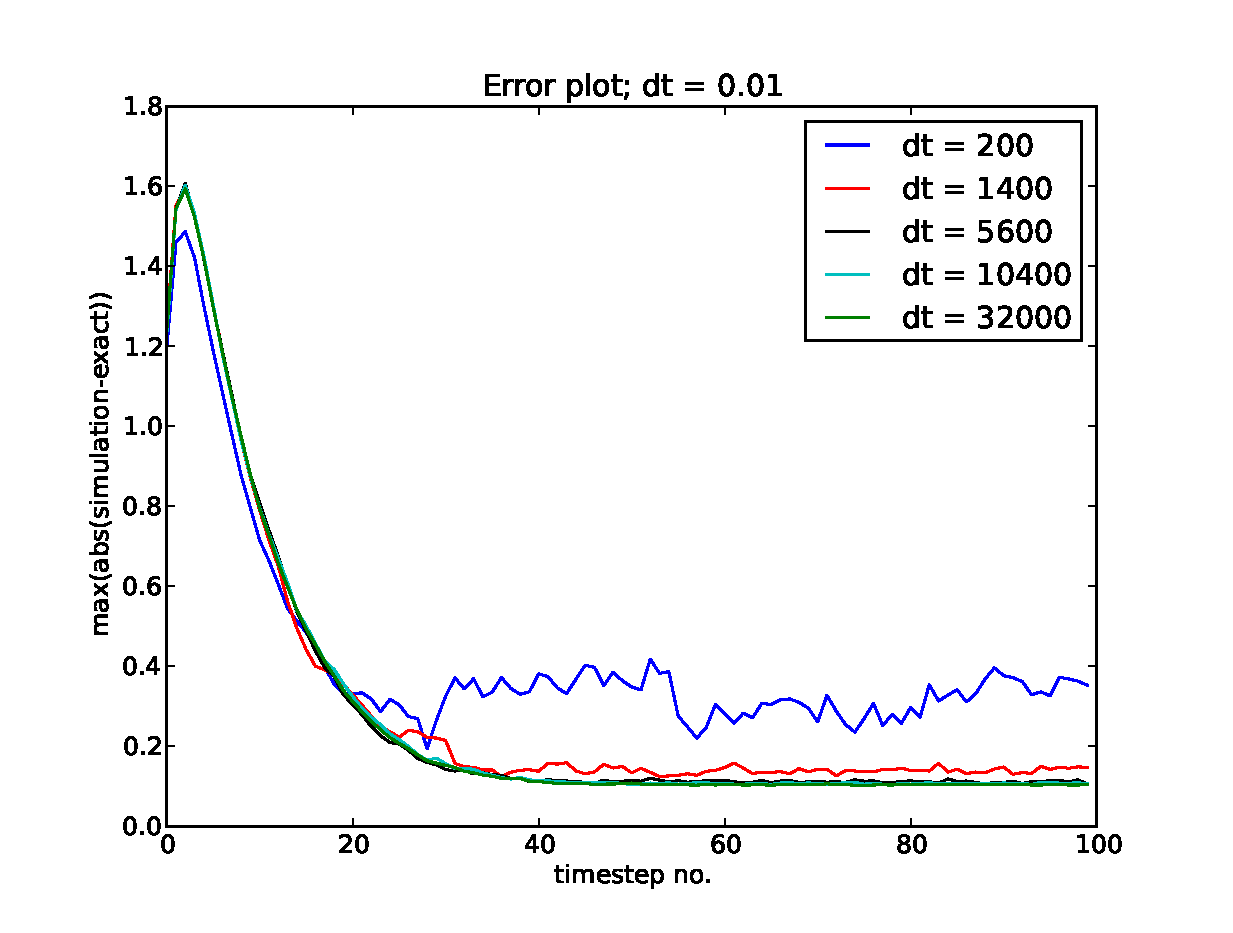
\includegraphics[scale=0.7]{../doc/results/experiment_18022014_1413_RW_convergencetest_1d/results/errorplot.eps}
 \caption[Error plot RW]{A ``normal'' error plot for the same simulation as in figure \ref{ConvergenceTestRW}. The $\Delta t$ in question is used to couple the RW simulation and the exact solution. For each $\Delta t$ the RW simulation does 100 steps with a step length calculated from equation \ref{steplength}}
\end{figure}




\section{Testing the combined solution}
In this chapter we will combine the PDE-solution on some part of the mesh with the result from a random walk simulation using the same initial condition as the PDE-solver was given. 
As we will discuss in chapter \ref{Software:About} there are many candidates as to the combination of the solutions, but we will use one of the simplest ones; the average of the two. 
Before we start with the verification, however, we will take a quick look at a simplified problem which in principle is the same.

\subsection{A simplified version of the algorithm}\label{simplified_test}

Monte Carlo methods are immensely important in modern computational science (\emph{reference}), and can be used to solve integrals as well as random walks. 
As a simplified analogy to our method for solving the diffusion equation we ca look to the Ordinary Differential Equation (ODE) in equation \ref{ODE}. 
\begin{equation}\label{ODE}
 \frac{\d f}{\d x} = a(x)\;\text{,}\; x\in [a,c]
\end{equation}
Equation \ref{ODE} is easily solvable (see eq. \ref{ODE_solution}), for the sake of illustration we also specify that $a(x) = \frac{1}{x}$ and divide the integral in two parts, introducing $b\in (a,c)$.
\begin{equation}\label{ODE_solution}
 f(x) = \int\limits_a^b a(x)\,dx + \int\limits_b^c a(x)\,dx
\end{equation}
This is a case where we have complete control over all parts of the solution which is $f(x) = f(b)-f(a) + f(c)-f(b)$, and we can solve the two parts of the integral in two different ways; by the midpoint method and by MC integration. The convergence rates of these methods are $2$ and $0.5$ respectively. 
By the relation we found earlier (eq. \ref{}) the number of MC samples should be proportionate to the resolution used by the midpoint-rule to the power of four. 
\begin{align*}
 \frac{1}{\sqrt{N}} \simeq \Delta x^2 \\
 N \simeq \frac{1}{\Delta x^4} = N_x^4
\end{align*}
The following output is from a program generously donated by Hans Petter Langtangen which does the required integration and calculates the convergence rates. 
It uses the relation described, but multiplies with a constant, giving us 
\begin{equation*}
 N = 2000\times N_x^4
\end{equation*}

\begin{lstlisting}
  N_x	    N_MC	   error       MC_error   MP_error
   1        2000 (   1)  2.650E-02   2.648E-02   2.391E-05
   2       32000 (   1)  7.392E-03   7.433E-03  -4.136E-05
   4      512000 (   1)  1.918E-03   1.927E-03  -8.954E-06
   8     8192000 (   8)  4.683E-04   4.866E-04  -1.832E-05
  16   131072000 ( 131)  1.176E-04   1.220E-04  -4.320E-06
  
  Convergence rates
total  MP     MC
-1.84 -1.83  0.20
-1.95 -1.95 -0.55
-2.03 -1.99  0.26
-1.99 -2.00 -0.52
\end{lstlisting}
We see that the convergence rate for the whole integral is roughly $2$ which is what we expect. This suggests that the idea behind the algorithm is sound. \\
Another thing to notice it the convergence rate of the MC method which is sort off all over the place, this illustrates how difficult it is to verify the simulations. 
As the listed output and equation \ref{} shows, the number of walkers or MC samples grows very fast making it computationally very demanding to do the calculations.

\subsection{Introducing walkers}

First of all, using random walkers on parts of the mesh will have a considerable, negative impact on the error estimate. 
As we have discussed before, the solution from the random walkers will fluctuate around the ``correct'' (it is in fact correct while verifying) solution with amplitude proportional to $\frac{1}{\sqrt{N_{ij}}}$ which will depend on the PDE-solution in the mesh-point. 
It will also, as demonstrated in chapter \ref{simplified_test}, be possible to force the combined solution to have the desired properties in terms of error-estimates but at considerable computational cost. 
While doing the various error-testing for the combined solution we will therefore stick to the implicit scheme since we can choose the time-step more freely and by extension reduce the number of random walkers required.\\
Keeping in mind that the spatial error goes like $\Delta x^2$ we should at least choose the time-step so that $\Delta t> \Delta x^2$ to make sure the error from the time derivative is dominant. 
Starting off, we have a 2d simulation of isotropic diffusion with $\Delta t = 0.01$ and $\Delta x = \frac{1}{75}$ over the full interesting course of the solution, meaning that the solution more or less at steady state the last time-steps. The error-plot from this simulation is shown in figure \ref{errorplot_combined_BE2d}. We can see that although the error-term from the combined solution does not converge onto the error-curve from the deterministic solution, the error term is of the same order. 
\begin{figure}[H]
 \centering
 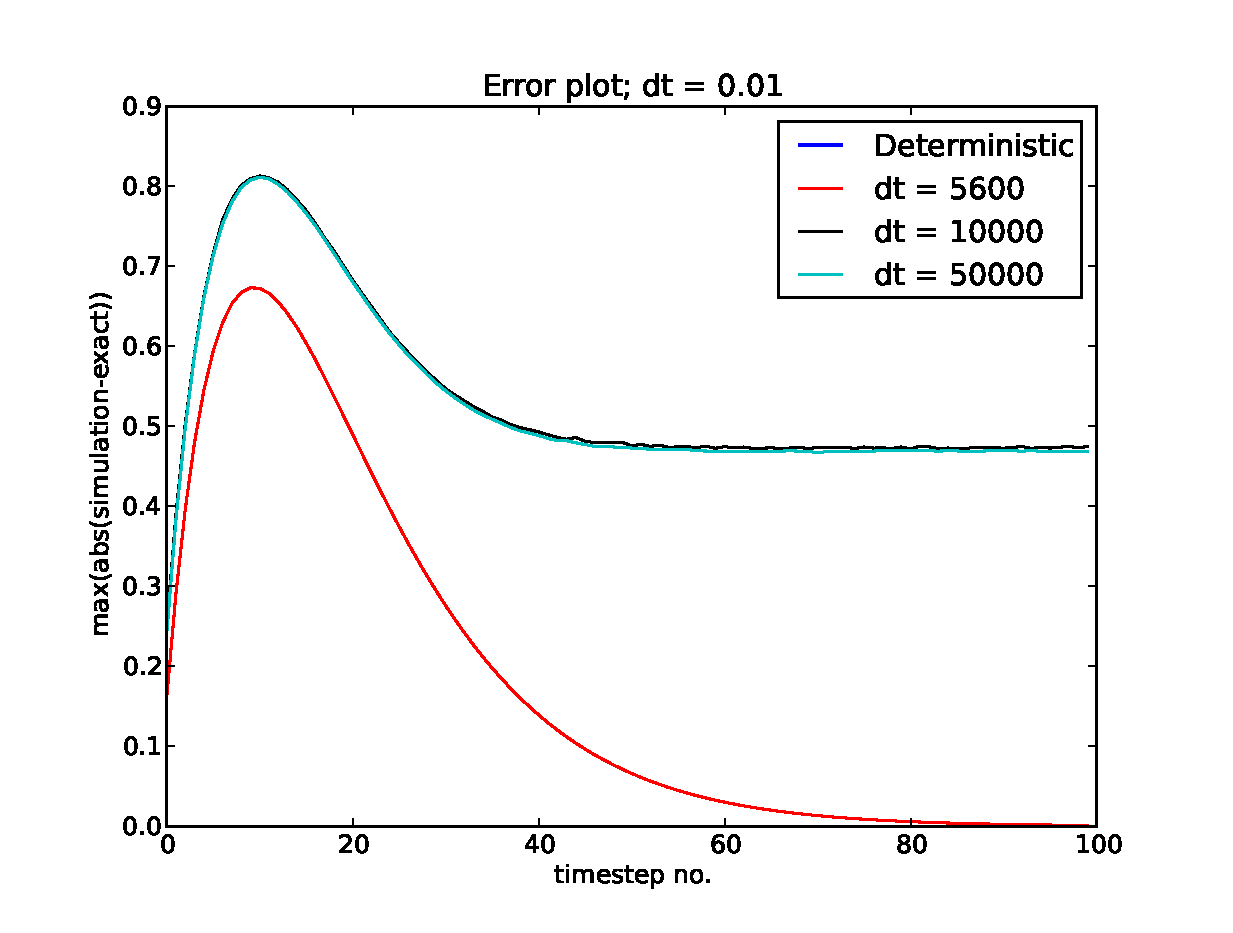
\includegraphics[scale=0.7]{../doc/results/experiment_17022014_1541/results/errorplot.eps}
 \caption{Error-plot of the combined solution using an increasing number of walkers. Parameters of importance are $\Delta t = 0.01$, $\Delta x = \frac{1}{75}$. Simulations doen with the BE scheme for 100 steps.}
 \label{errorplot_combined_BE2d}
\end{figure}


We then introduce an area on the domain where we switch models from the normal PDE to an average of the PDE solution and the result of a random walk simulation where the initial condition is the last time step from the PDE converted to walkers by the conversion rate given in equation \ref{conversion_rate}. In this case we have used the parameters $a=3$, $\Delta t = \frac{\Delta x^2}{3.0}$, $\Delta x = \frac{1}{20}$. 
These parameters makes one unit of $u(x,t)$ equal to some $1000$ walkers. 
\begin{equation}\label{conversion_rate}
 C_{ij} = \frac{a}{\Delta t}U_{ij}
\end{equation}
Mostly we will rewrite equation \ref{conversion_rate} to just one conversion factor times the PDE solution, giving us some flexibility should we want to add more dependencies in the conversion. 
As of now, the conversion factor, $Hc$, is defined in equation \ref{definition_Hc_first}. 
One ``unit'' of $ U_{ij}$ will directly correspond to $Hc$ random walkers.
\begin{equation}\label{definition_Hc_first}
 Hc =  \frac{a}{\Delta t} \implies C_{ij} = Hc\cdot U_{ij}
\end{equation}

The area where the model has been replaced is between $x=0.6$ and $x=0.7$, which is three mesh points. 
In the same way as for only the simple 1D PDE case we compare the combined numerical solution from the two models to the exact solution. 
Figure \ref{errorplot_FE1D_Walk_first_attemt} shows that the error is still of the order of $\Delta t$, and the difference between the two models are negligible. 

\begin{figure}[H]
\centering
\includegraphics[scale=0.7]{../doc/results/experimen(t_i)t_31102013_1017/results/errorplot.eps}
\caption[Effect of increasing number of walkers]{Numerical error for 1D Forward Euler discretization combined with random walk model between $x=0.6$ and $x=0.7$. Other parameters of importance are $\Delta t\approx 0.00083333$, $\Delta x = 0.05$.}
\label{errorplot_FE1D_Walk_first_attemt}
\end{figure}

As we can see from figure \ref{errorplot_FE1D_Walk_first_attemt} increasing the number of walkers that each ``unit concentration'' corresponds to has a positive effect on the error norm up to a certain point. 
After we reach $Hc \sim 10^4$ the error is dominated by the truncation error of the Forward Euler scheme. 
This tells us that the error associated with introducing a random walk model on parts of the mesh behaves roughly as we hoped; it tends to zero for large numbers of walkers. 
Meaning of course that the calculations in section \ref{} are not hopeless.


\subsection{Increasing the time step and the relative size of walk-area}\label{increasing_dt}

Now that we have an estimate of how to adjust the step length of the walkers in order to adjust for the time step, $\Delta t$, on the PDE level we would like to investigate the actual effects of running the simulation with a larger time step to verify our calculations. 
First off all, figure \ref{errorplot_BE1D_noWalk} shows the error norm of a simulation of the simplest diffusion equation \ref{simple_diffusion_equation} discretized by the Backward Euler scheme \ref{BE_discretisation_isotropic} using a time step which would make the Forward Euler discretization unstable (There is something strange about its convergence). 
Figure \ref{errorplot_BE1D_Walk} shows the same simulation for various conversion parameters for the random walk. 
These simulations have input from the random walk model on some 20\% of the mesh points. 
As a comparison we can turn to figures \ref{errorplot_BE1D_walk_5_percent} and \ref{errorplot_BE1D_walk_35_percent} which have 5\% and 35\% of the mesh points affected by walkers.

\begin{figure}[H]
\centering
\begin{subfigure}[b]{0.48\textwidth}
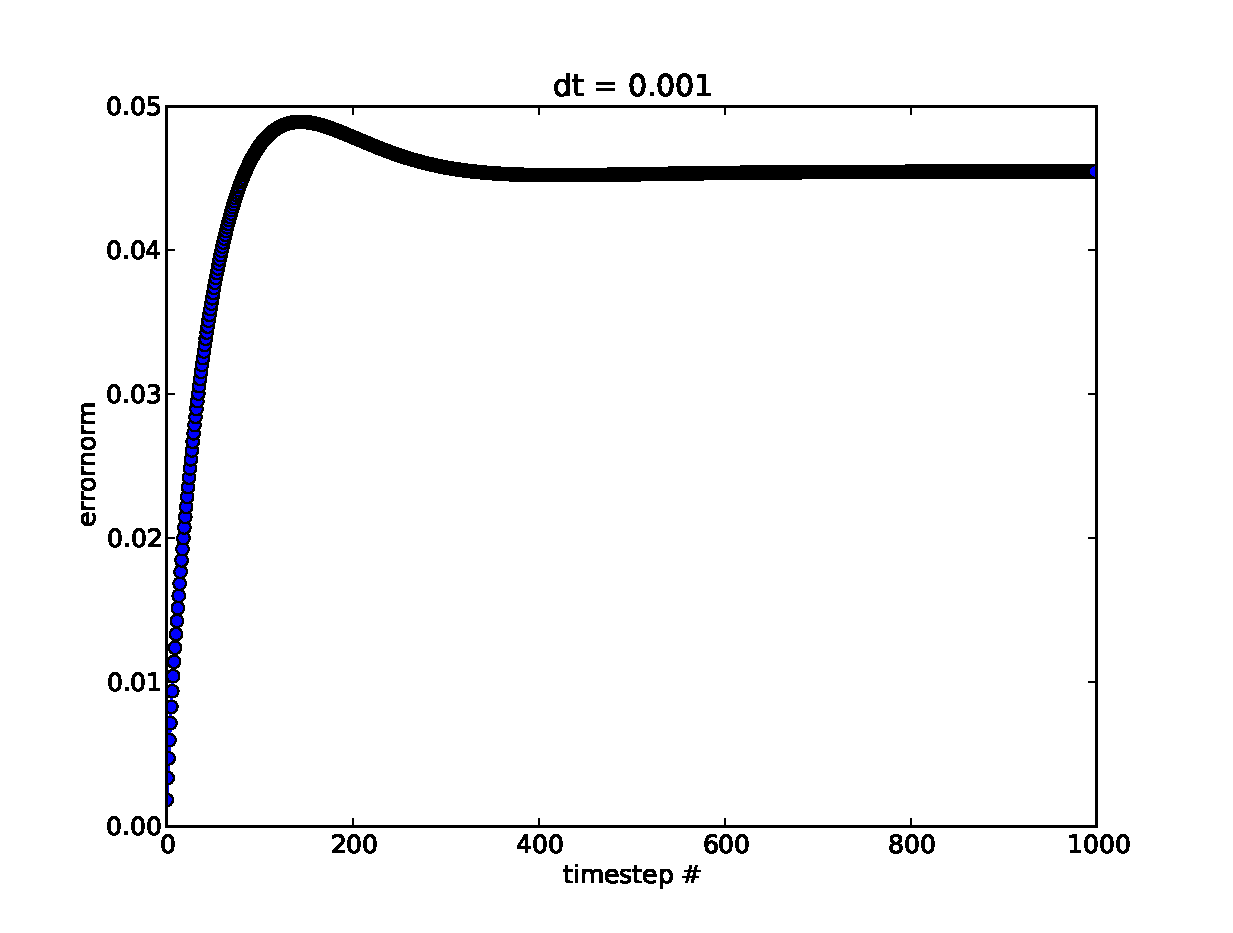
\includegraphics[width=\textwidth]{../doc/results/experiment_19112013_1514/results/deterministic_errorplot.eps}
\caption{}
\label{errorplot_BE1D_noWalk}
\end{subfigure}
\begin{subfigure}[b]{0.48\textwidth}
 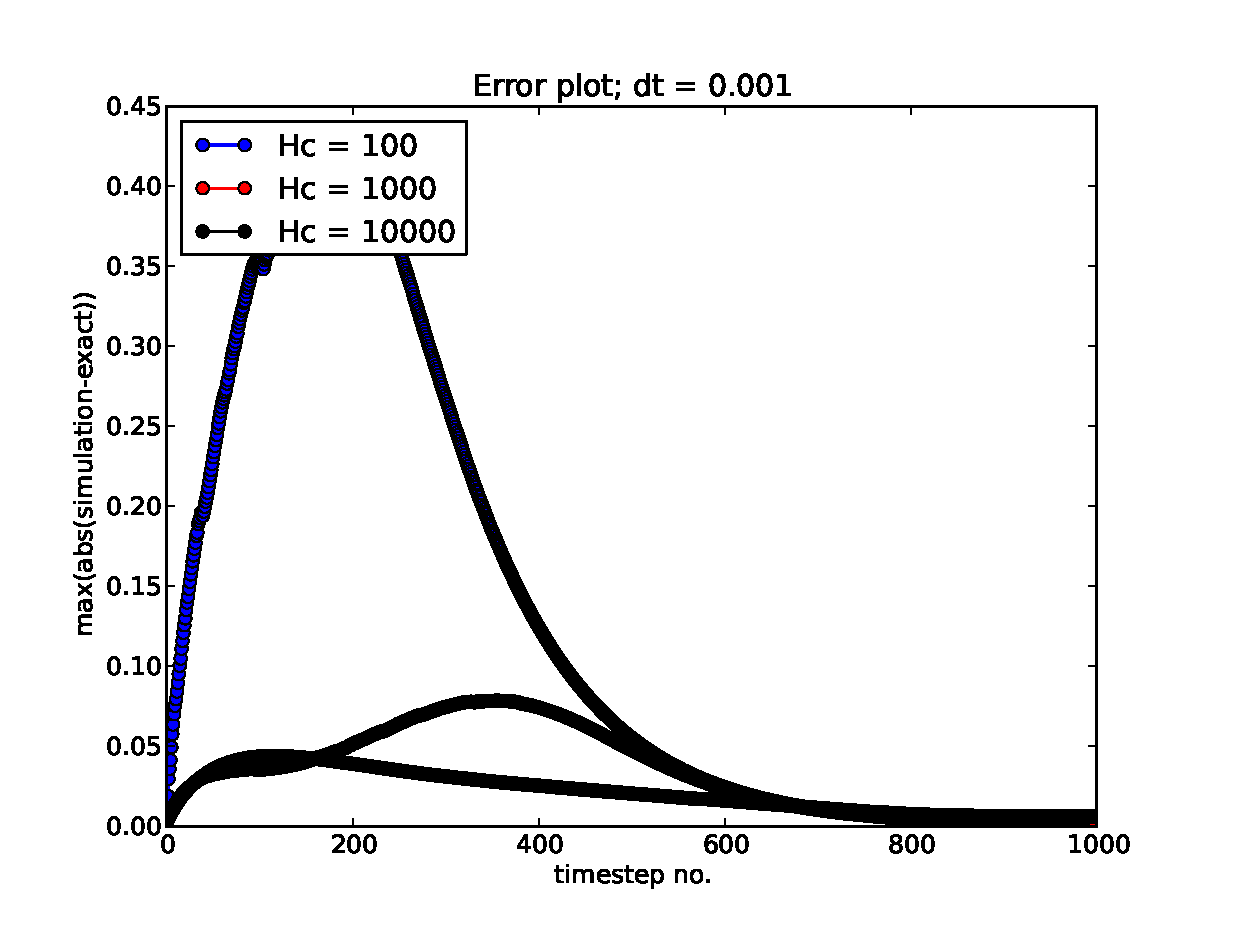
\includegraphics[width=\textwidth]{../doc/results/experiment_19112013_1514/results/errorplot.eps}
 \caption{}
 \label{errorplot_BE1D_Walk}
\end{subfigure}
\caption[Numerical error for 1D Backward Euler discretization]{Numerical error for 1D Backward Euler discretization of the PDE. In figure b there has been added walkers to the solution in the area $x\in[0.5,0.7]$.}
\label{errorplot_BE1D_first}
\end{figure}

\begin{figure}[H]
\centering
\begin{subfigure}[b]{0.48\textwidth}
 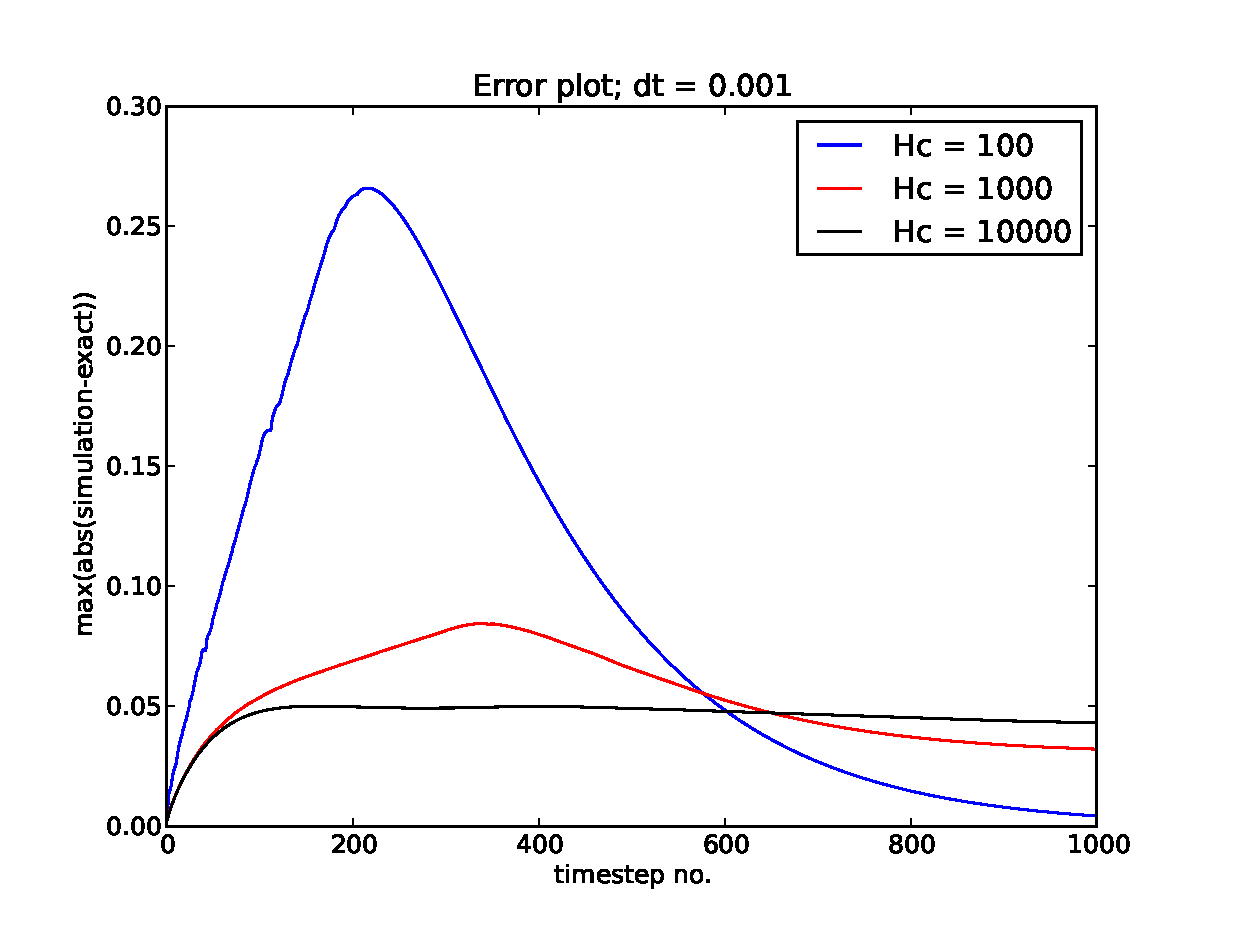
\includegraphics[width=\textwidth]{../doc/results/experiment_19112013_1559/results/errorplot.eps}
 \caption{Having walkers on 5\% of the mesh points.}
 \label{errorplot_BE1D_walk_5_percent}
\end{subfigure}
\begin{subfigure}[b]{0.48\textwidth}
 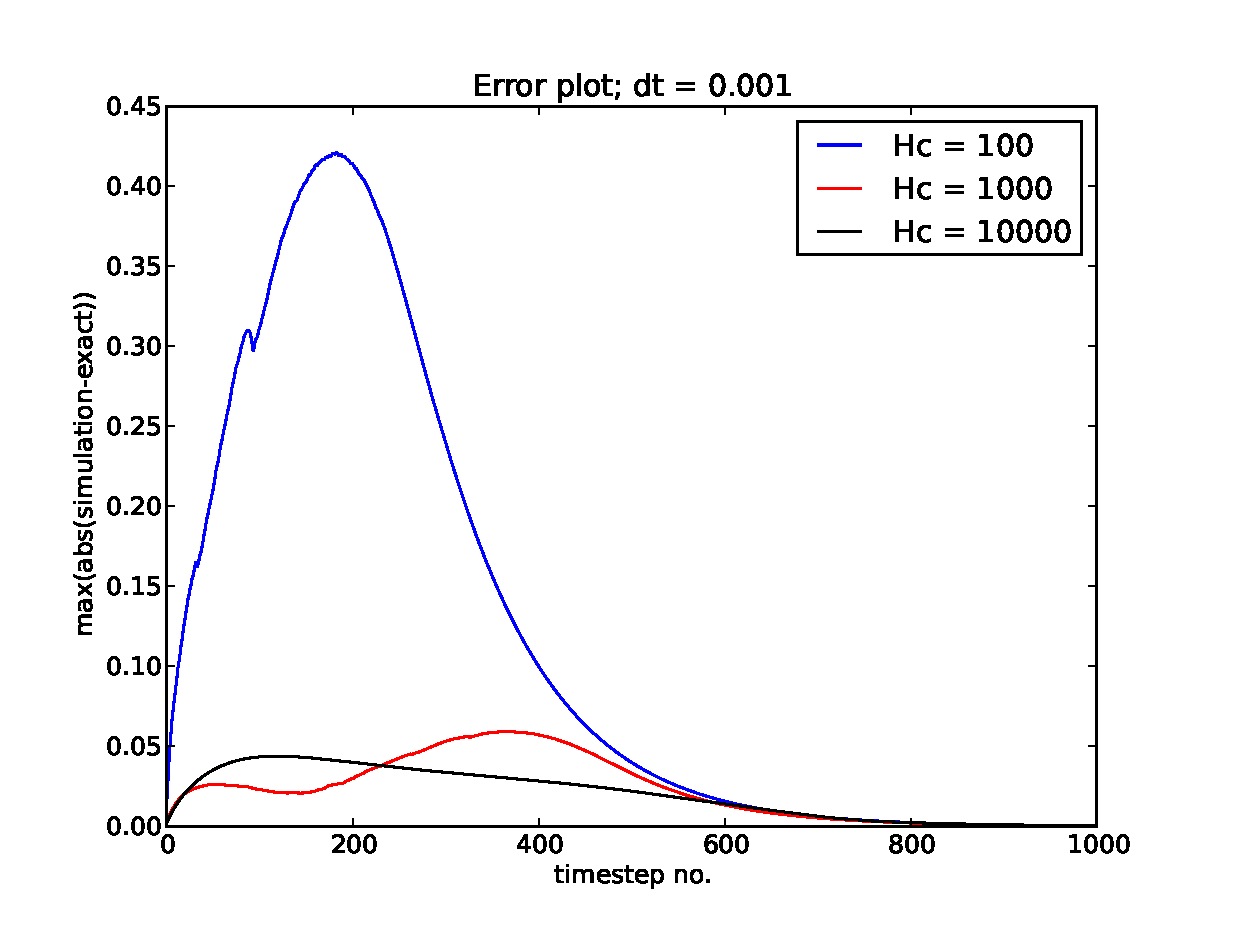
\includegraphics[width=\textwidth]{../doc/results/experiment_19112013_1603/results/errorplot.eps}
 \caption{Having walkers on 35\% of the mesh points.}
 \label{errorplot_BE1D_walk_35_percent}
\end{subfigure}
\caption{The effect of increasing the size of the walk area for a fixed $\Delta t = 0.001$ using the BE discretization.}
\label{testing_walk_area_size_BE}
\end{figure}

These experiments have been done using the Backward Euler discretization so that we can simulate for a longer time and still see the effects to their full extent. 
We have also investigated the effects of changing the time step (also using the BE discretization to avoid instabilities and be able to do longer simulations). 
The results are summarized in figure \ref{testing_dt_size}. 
We notice something a bit unexpected in figure \ref{errorplot_BE1D_walk_large_dt}. 
Unlike almost all the other comparable plots, it seems that using the least amount of walkers gives the best result here. 
This might be because the system quickly reaches its steady state, and will then be very well described by the continuum model. 
Having a small conversion factor, Hc, will mean that very quickly there will be no walkers which sort of ruins the point. 
This particular equation has steady state $u(t\to\infty,x) = 0$, and so not having any walkers will be perfect. What we should read from this figure is rather that the simulation with the most walkers converges to an acceptable error, and that this is achieved just as fast as for the other two simulations.



\begin{figure}[H]
\centering
\begin{subfigure}[b]{0.48\textwidth}
 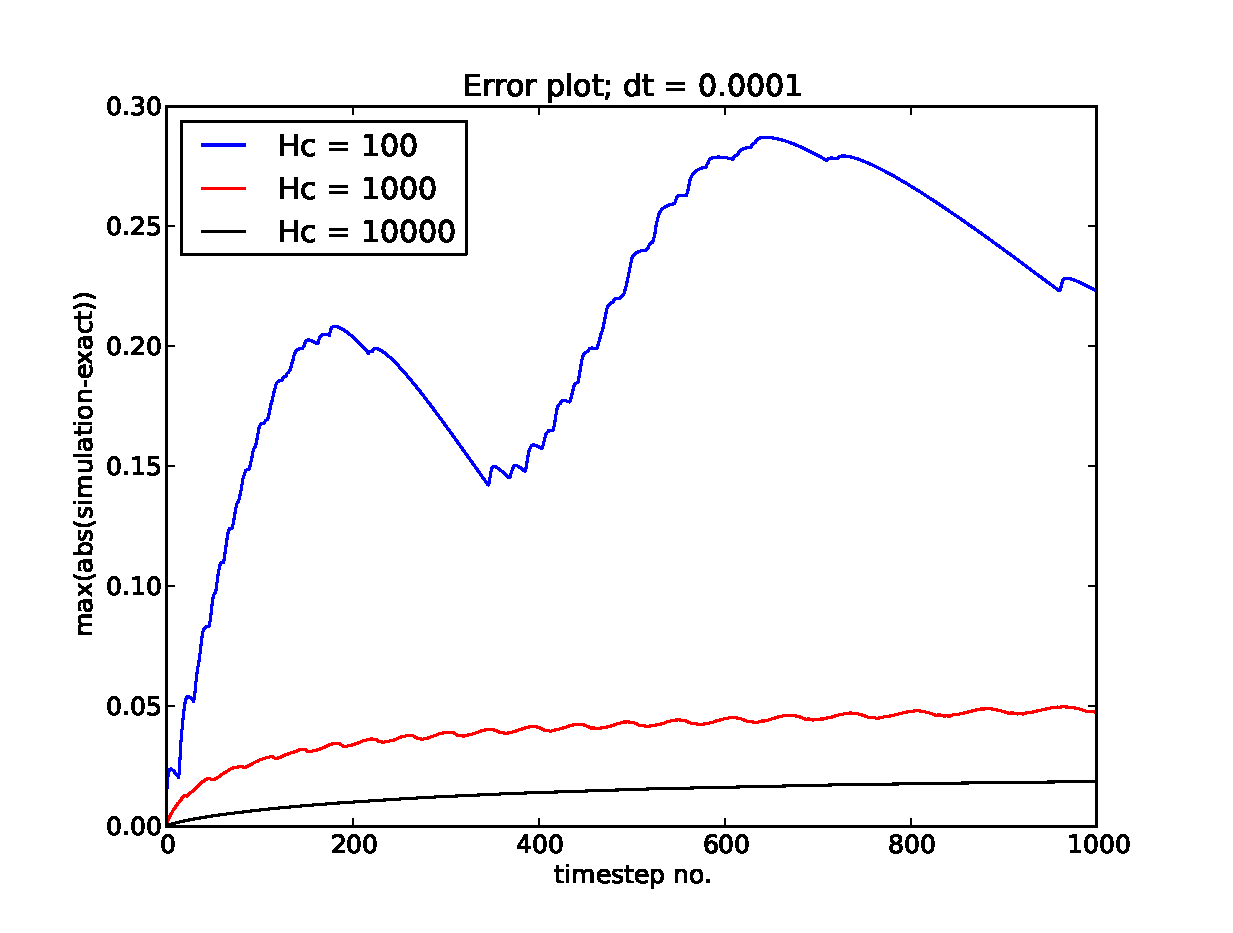
\includegraphics[width=\textwidth]{../doc/results/experiment_19112013_1625/results/errorplot.eps}
 \caption{Using a normal $\Delta t = 0.0001$.}
 \label{errorplot_BE1D_small_dt}
\end{subfigure}
\begin{subfigure}[b]{0.48\textwidth}
 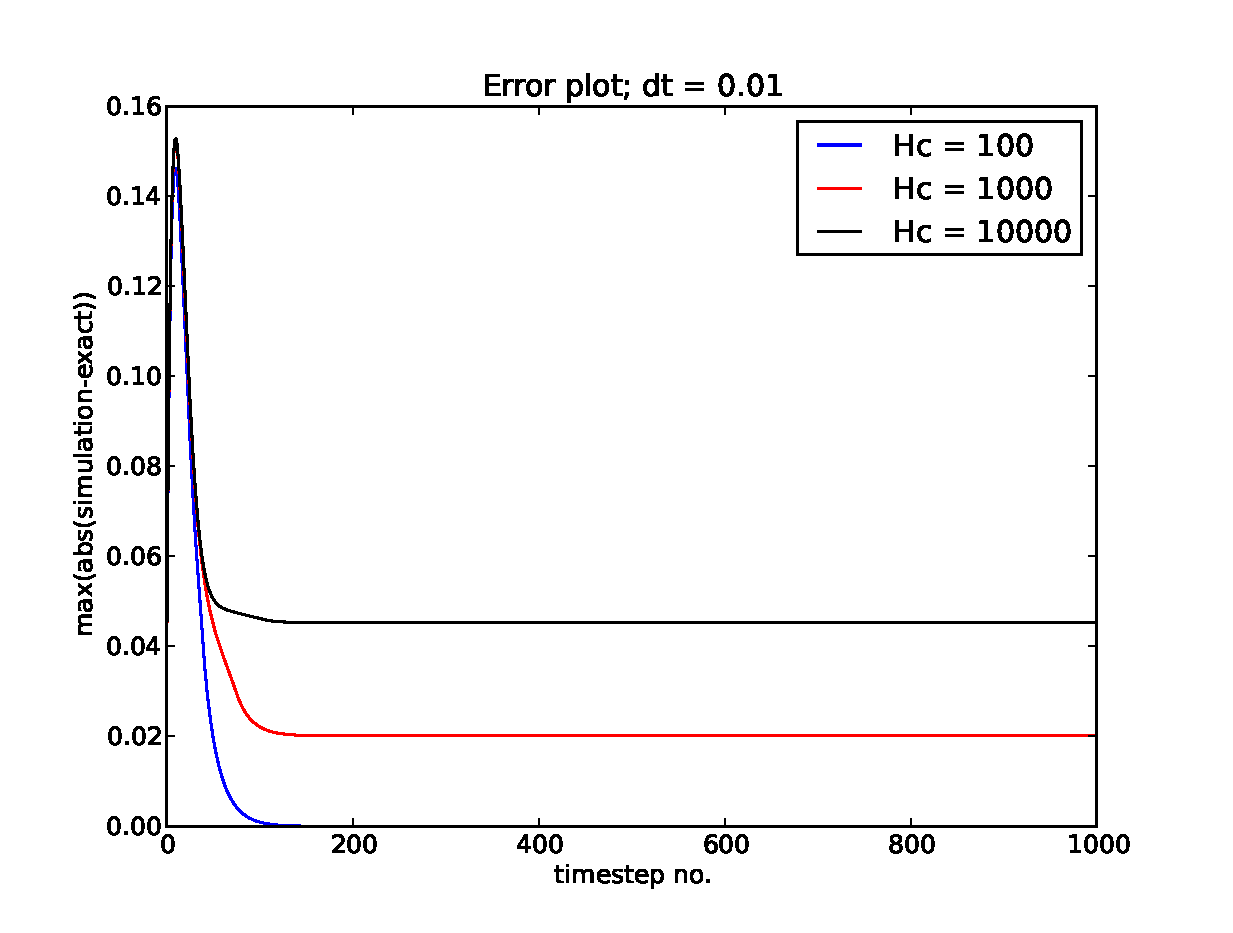
\includegraphics[width=\textwidth]{../doc/results/experiment_19112013_1627/results/errorplot.eps}
 \caption{Using a large $\Delta t = 0.01$.}
 \label{errorplot_BE1D_walk_large_dt}
\end{subfigure}
\caption{}
\label{testing_dt_size}
\end{figure}

\begin{figure}[H]
 \centering
\begin{subfigure}[b]{0.48\textwidth}
\includegraphics[width=\textwidth]{{../doc/results/experiment_02122013_1309_long_simulations_1d/results/errorplot}.eps}
 \caption{}
 \label{errorplot_FE_walk_long:normal}
\end{subfigure}
\begin{subfigure}[b]{0.48\textwidth}
 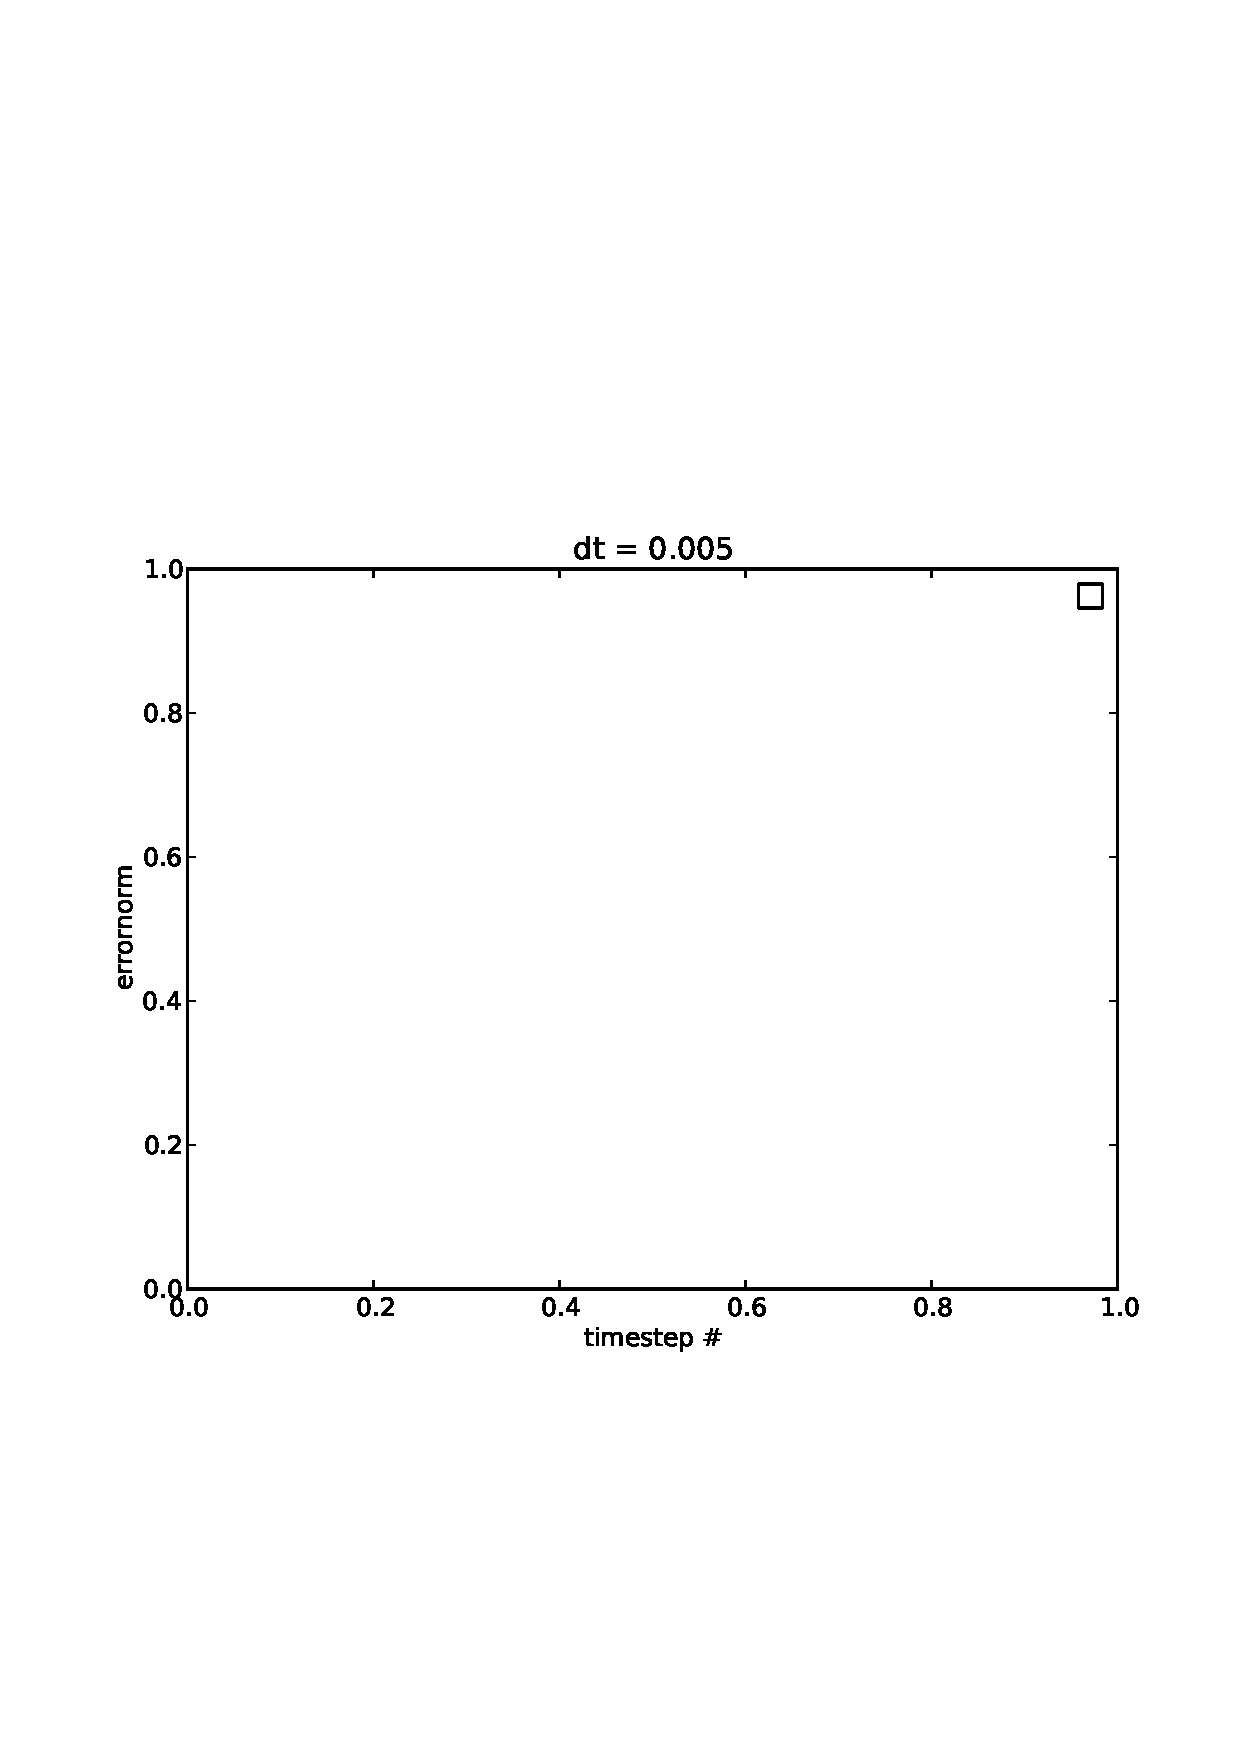
\includegraphics[width=\textwidth]{{../doc/results/experiment_02122013_1309_long_simulations_1d/results/deterministic_errorplot}.eps}
\caption{}
\label{errorplot_FE_walk_long:deterministic}
 \end{subfigure}
\caption[Errorplot, long simulation]{The deterministic errory

 Current goal:
Beat Brock, then head to Mt Moon. and the error from simulations with walkers for long simulations.}
\label{errorplot_FE_walk_long}
\end{figure}

\subsection{The effects of adding drift to the walkers}\label{effect_of_drift_on_walkers}

As shown in section \ref{random_walks_and_drift} adding drift to the walkers will modify our model to represent the convection diffusion equation (\ref{convection_diffusion_equation}) rather than the simple diffusion equation. 
In our analysis so far we have completely ignored the spatial truncation error because it is of second order, and the truncation error in time is of first order. 
When discretizing the convection diffusion equation however, we must take care to use an approximation to the first order spatial derivative that has a truncation error of second order. 

Otherwise the truncation error in this term will completely dominate seeing as $\Delta t<\Delta x$. 
We must also find a new stability criterion for the scheme. \\
As for now, the Leap-frog discretization will do (though it is not by far a perfect choice seeing as it is unstable). 
As a side note we can also note that the Neumann boundary condition will be very clear in this scheme. 
$\frac{\d C}{\d n} = 0 \implies \frac{\d C}{\d x} = 0 $ on the boundary, leading to $C_{-1} = C_{1}$ on the boundary and canceling the drift term on the boundary.
\begin{equation}\label{convection_diffusion_equation_leapfrog}
 C^{n+1} = \frac{D\Delta t}{\Delta x^2}\left(C^n_{i+1}-2C^n_i+C^n_{i-1}\right)-\frac{v\Delta t}{2\Delta x}\left(C^n_{i+1}-C^n_{i-1}\right) + C^n
\end{equation}
The truncation error for the first order derivative using the Leap-frog scheme is obtained as follows
\begin{align*}
 u(t,x+\Delta x) = u(t,x) + \frac{\d u(t,x)}{\d x}\Delta x + \frac{\d^2u(t,x)}{2\d x^2}\Delta x^2 +\mathcal{O}(\Delta x^3)\\
 u(t,x-\Delta x) = u(t,x) - \frac{\d u(t,x)}{\d x}\Delta x + \frac{\d^2u(t,x)}{2\d x^2}\Delta x^2 +\mathcal{O}(\Delta x^3)
\end{align*}
which we recognize as the same error we got from the second order spatial derivatives.\\
If we now do the same analysis as we have already done, by finding a manufactured solution to the convection diffusion equation, implementing a numerical scheme like \ref{convection_diffusion_equation_leapfrog} to solve it after and taking the error norm. \\
The error norm does not have to go as $\Delta t$, but it must be halved (approximately) if we halve $\Delta t$. 
Figure \ref{} shows two simulations of equation \ref{convection_diffusion_equation} for $D =1$ and $v=1$ compared to the manufactured solution \ref{manifactured_solution_1D} without adding walkers. 
Before the simulation we must find a source term so the manufactured solution will solve the equation.
\begin{align*}
 -\pi^2\exp\left(-\pi^2t\right)\cos\left(\pi x\right) &= -\pi^2D\exp\left(-\pi^2t\right)\cos\left(\pi x\right) + \pi v \exp\left(-\pi^2t\right)\sin\left(\pi x\right) + f(x,t)\\
 -\pi^2\cos\left(\pi x\right) &= \pi^2D\cos\left(\pi x\right) +\pi v \sin\left(\pi x\right) + \tilde{f}(x) \\
 \tilde{f}(x) &= -\pi\sin\left(\pi x\right)
\end{align*}
Where $f(x,t) = \exp\left(-\pi^2t\right)\tilde{f}(x)$.

\begin{figure}[H]
\centering
\begin{subfigure}[b]{0.48\textwidth}
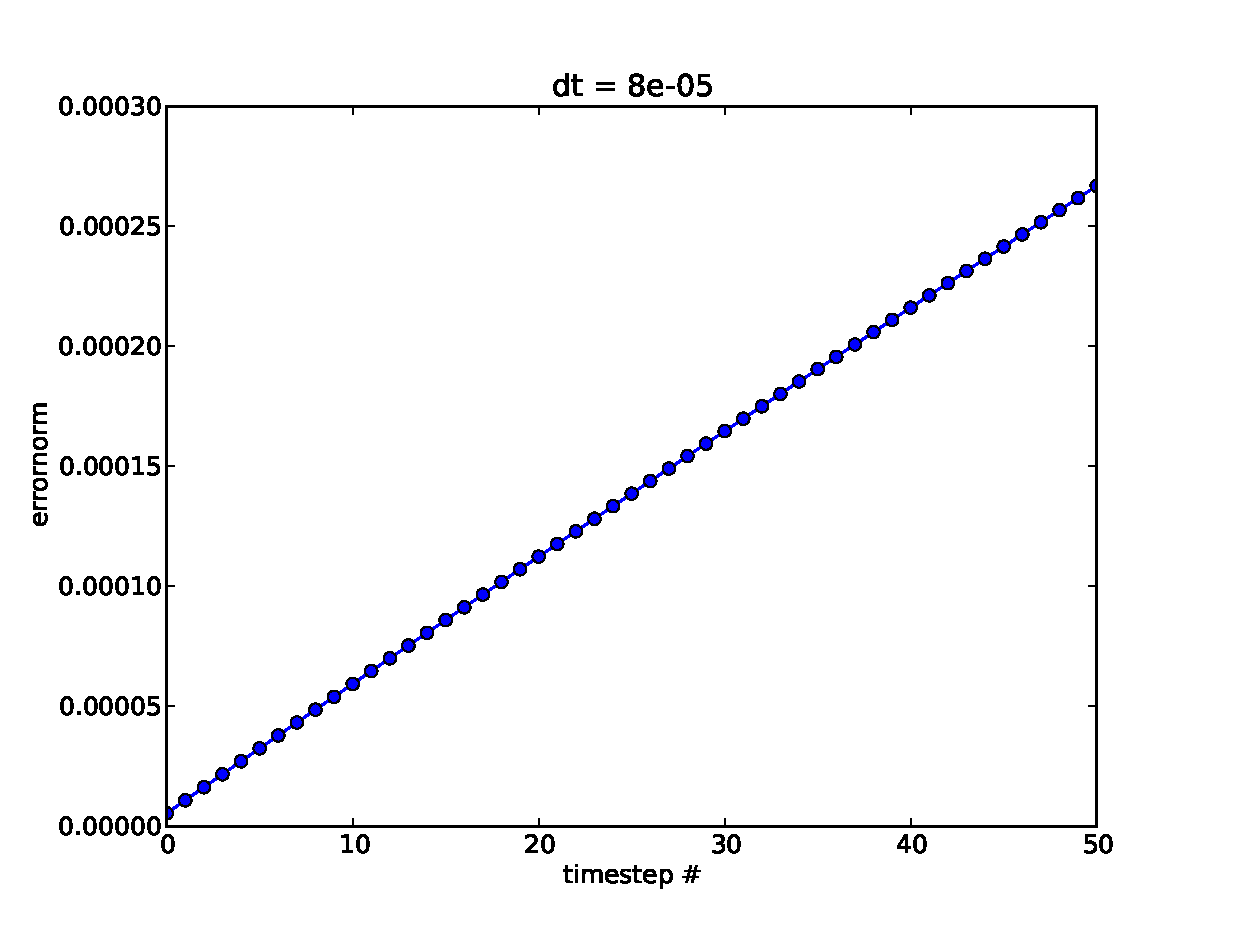
\includegraphics[width=\textwidth]{../doc/results/experiment_05112013_1235/results/deterministic_errorplot.eps}
\caption{}
\label{Verification_convection_diffusion:single_dt}
\end{subfigure}
\begin{subfigure}[b]{0.48\textwidth}
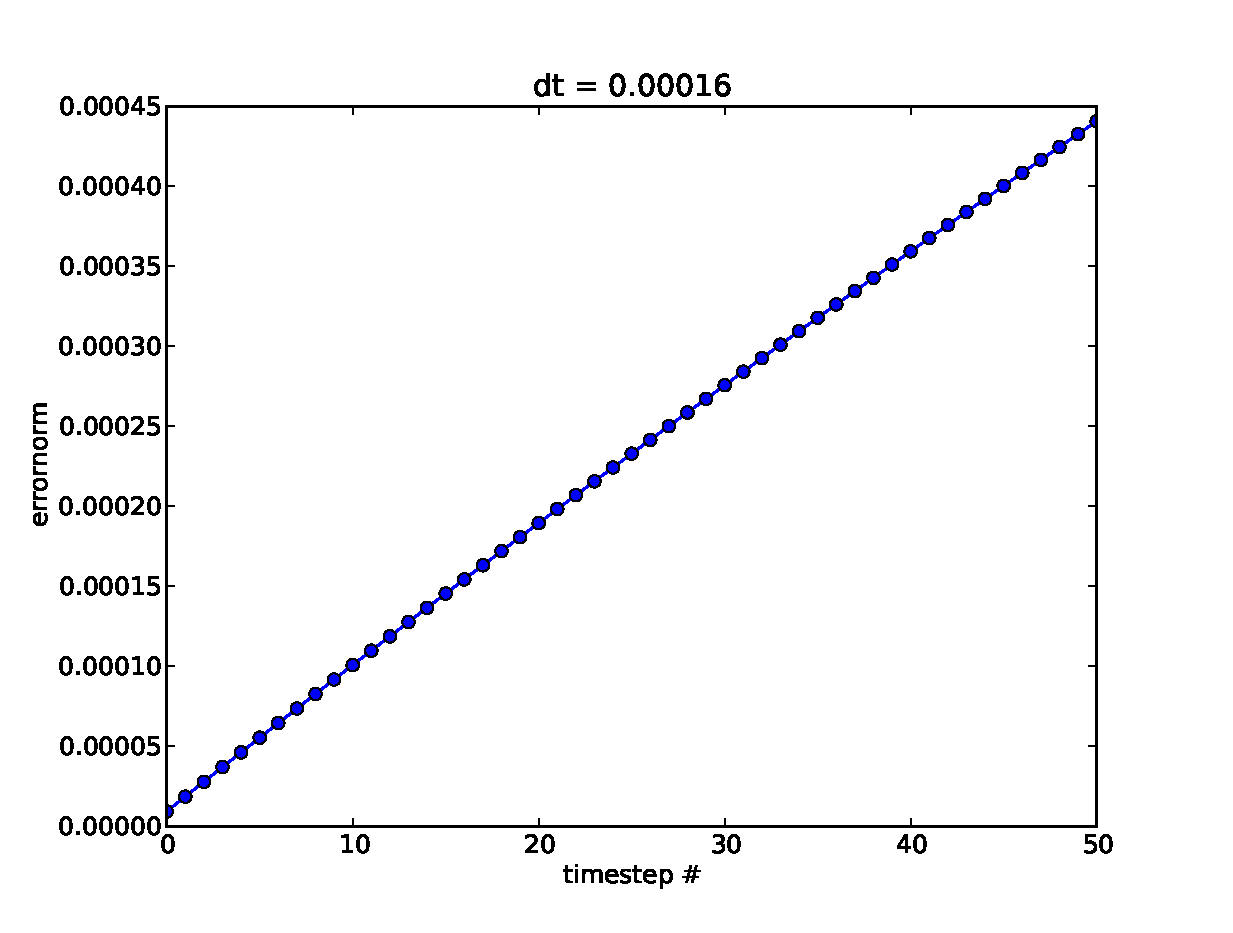
\includegraphics[width=\textwidth]{../doc/results/experiment_05112013_1234/results/deterministic_errorplot.eps}
\caption{}
\label{Verification_convection_diffusion:double_dt}
\end{subfigure}
\caption[Verification of Convection diffusion equation implementation]{Verification of Convection diffusion equation implementation}
\label{Verification_convection_diffusion}
\end{figure}

As we see from figure \ref{Verification_convection_diffusion} the error norm is halved when $\Delta t$ is roughly halved, just as we expected. It is also of the order of $\Delta t$, which is nice.  
We can then advance to testing the effect of adding an area of walkers for different values of $Hc$ as before. 
Note that we can no longer use the manufactured solution now if we wish to add drift to the walkers because we have forced the solution to fit the equation by tampering with the source term. 
The effect of
\begin{figure}[H]
\centering
\begin{subfigure}[b]{0.48\textwidth}
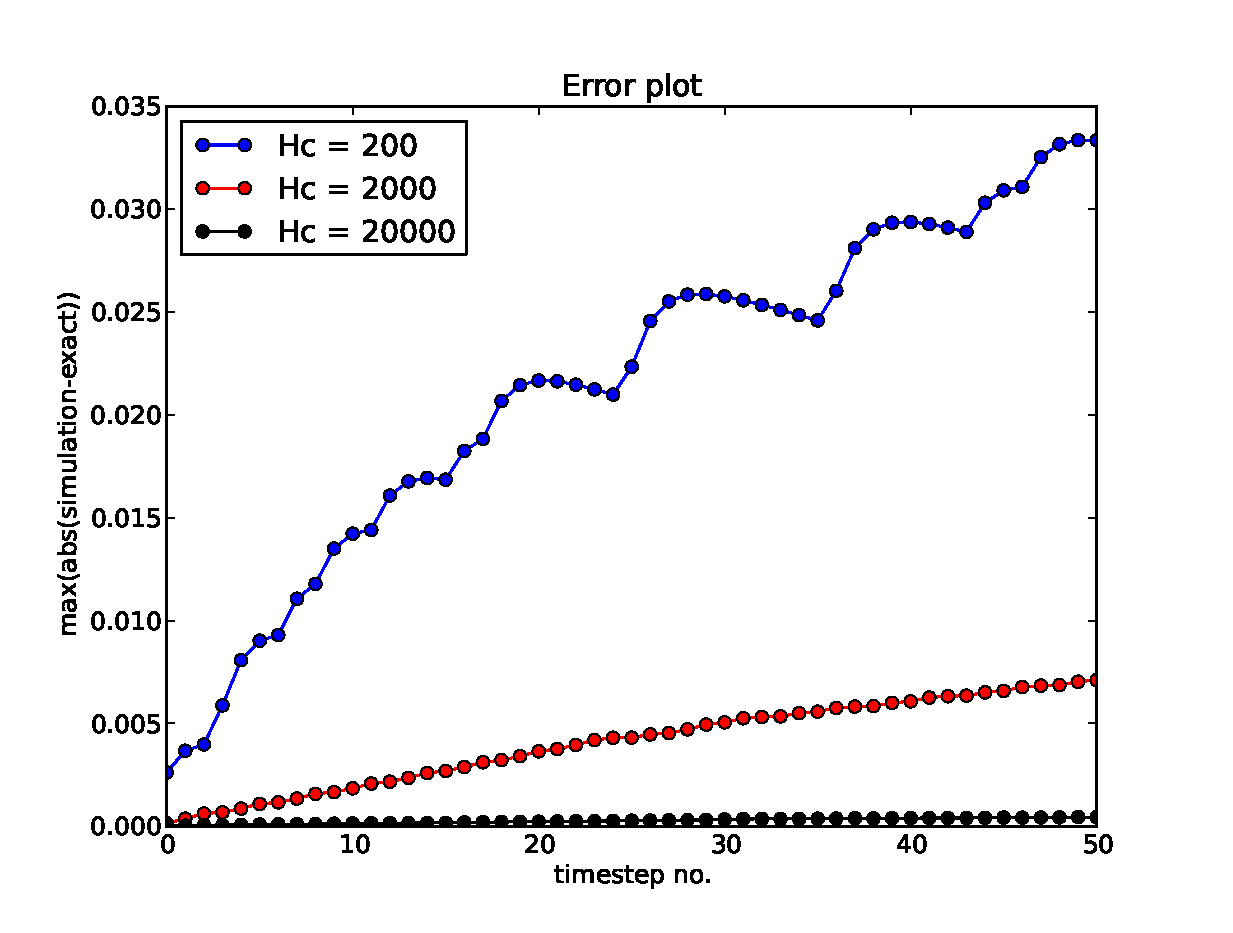
\includegraphics[width=\textwidth]{../doc/results/experiment_05112013_1237/results/errorplot.eps}
\caption{}
\label{Errortest_convection_diffusion_walkers:few_walkers}
\end{subfigure}
\begin{subfigure}[b]{0.48\textwidth}
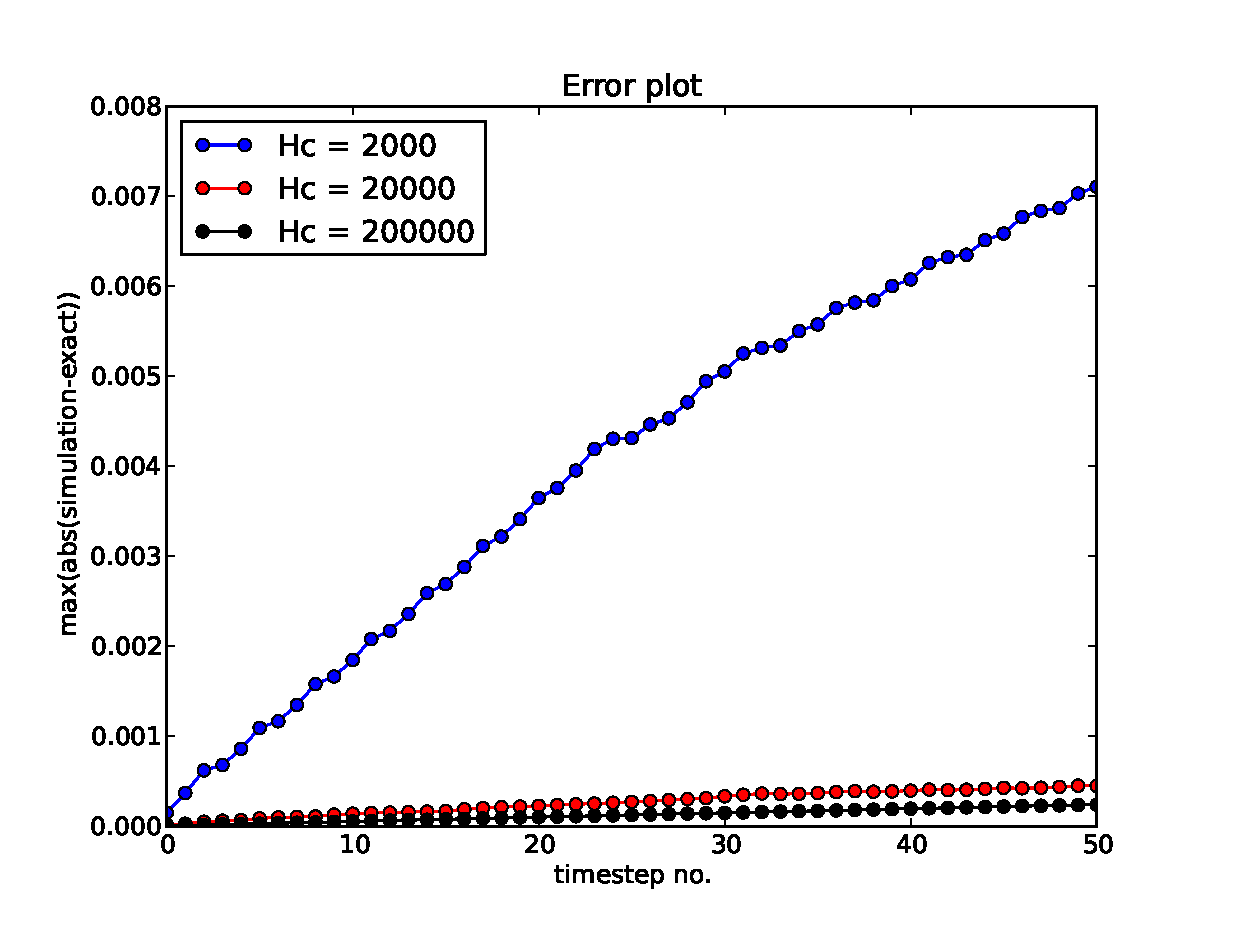
\includegraphics[width=\textwidth]{../doc/results/experiment_05112013_1239/results/errorplot.eps}
\caption{Adding more walkers still has the desired effect on the error, suggesting that the central limit theorem is at work behind the scenes.}
\label{Errortest_convection_diffusion_walkers:more_walkers}
\end{subfigure}
\caption[Adding walkers influenced by drift]{The figure shows the effect adding walkers influenced by drift has on the error. 
The drift term is the step length, which is quite large. The strangest thing is, however, that changing the direction of the drift has little effect on the error, suggesting that the drift term is completely wrong in relation to the steplength. $\Delta t =8e-5$}
\label{Errortest_convection_diffusion_walkers}
\end{figure}



